%% MDPI Remote Sensing LaTeX submission -- generated by scripts/build_latex_mdpi.py
%% Do not edit by hand; edit manuscript/draft_mdpi.md and rebuild.
%% NB: the 'pdftex' class option from MDPI's template is intentionally omitted
%% so xcolor/graphicx auto-detect the driver -- we compile with tectonic (XeTeX),
%% under which the pdftex driver's \pdfcolorstack is undefined. MDPI compiles
%% the accepted paper with pdfLaTeX at production; the source remains valid there.
\documentclass[remotesensing,article,submit,moreauthors]{Definitions/mdpi}
\usepackage{amssymb} % \lesssim, \gtrsim etc. (mdpi.cls loads amsmath only)
\usepackage{adjustbox} % shrink over-wide tables to \textwidth

\firstpage{1}
\makeatletter
\setcounter{page}{\@firstpage}
\makeatother
\pubvolume{1}
\issuenum{1}
\articlenumber{0}
\pubyear{2026}
\copyrightyear{2026}
\datereceived{ }
\dateaccepted{ }
\datepublished{ }
\hreflink{https://doi.org/}

% pandoc emits these helpers in its standalone template; we paste fragments,
% so define them here (no-ops / minimal) to keep the body self-contained.
\providecommand{\tightlist}{\setlength{\itemsep}{0pt}\setlength{\parskip}{0pt}}
\providecommand{\passthrough}[1]{#1}

\newcommand{\orcidauthorA}{0000-0002-4111-8959}
\newcommand{\orcidauthorB}{0000-0002-2534-3777}

\Title{Predicting Tidal-Sampling Bias of Sun-Synchronous Satellites from
Overpass Phase: Theory and Validation on Macrotidal Coasts}
\TitleCitation{Predicting Tidal-Sampling Bias of Sun-Synchronous Satellites from
Overpass Phase: Theory and Validation on Macrotidal Coasts}

\Author{Taeyoon Song $^{1,2,}$*\orcidA{} and Mirinae Kim $^{2}$\orcidB{}}
\AuthorNames{Taeyoon Song and Mirinae Kim}
\AuthorCitation{Song, T.; Kim, M.}

\address{%
$^{1}$ \quad Department of Ocean Sciences, Inha University, Incheon 22212, Republic of Korea\\
$^{2}$ \quad Haebom Data Inc., \#904, Gasan A1 Tower, 205-27 Gasan 1-ro, Geumcheon-gu, Seoul 08503, Republic of Korea; tysong@haebomdata.com (T.S.); mirinae@haebomdata.com (M.K.)}

\corres{Correspondence: tysong@haebomdata.com}

\abstract{The waterline method for mapping intertidal digital elevation models
(DEMs) from optical satellite imagery assumes that scenes sample the
local tidal cycle without systematic bias. We derive a closed-form model
in which the satellite-sampled tide bias equals
\(\beta \cdot A \cdot \langle\cos\theta\rangle\), where \(A\) is the
local tidal amplitude and \(\langle\cos\theta\rangle\) the mean cosine
of the overpass tide phase, and validate it over the macrotidal Korean
coast using 5,082 cloud-screened Landsat-8/9 and Sentinel-2 acquisitions
(2020--2024) at five tidal flats against hourly tide-gauge observations.
Sun-synchronous satellites sample only 70--80 \% of the astronomical
tidal envelope, systematically missing one extremity. The resulting mean
bias has opposite signs on the macrotidal west coast (low-tide bias) and
the southern amphidromic coast (high-tide bias). A single slope
\(\beta = 1.78\) reproduces the bias across five sites and three sensors
(\(R^{2} = 0.98\)) and is recovered from the global FES2022b tide model
alone (\(R^{2} = 0.983\)), enabling correction without local gauge data.
The bias yields an elevation-domain RMSE of 0.36--1.09 m and unsampled
intertidal bands up to 2.5 km wide; because all optical missions cluster
near 10:30 local solar time, only phase-orthogonal radar --- not higher
optical revisit frequency --- can close the gap.}

\keyword{tidal flat; intertidal DEM; waterline method; tidal aliasing; sun-synchronous orbit; amphidromic system}

\begin{document}

\subsection*{Highlights}\label{highlights}
\addcontentsline{toc}{subsection}{Highlights}

\begin{itemize}
\tightlist
\item
  Closed-form bias = \(\beta \cdot A \cdot \langle\cos\theta\rangle\)
  explains 98 \% of cross-sensor variance
\item
  Bipolar tide-bias sign reverses across the Korean amphidromic phase
  gradient
\item
  \(\beta > 1\) decomposes into a spring--neap \ensuremath{\times} overpass-phase
  covariance diagnostic
\item
  FES2022b global model reproduces the fit; no local tide-gauge data
  required
\item
  Yields 0.4--1.1 m DEM error and up to 2.5 km of permanently unsampled
  flats
\end{itemize}

\subsection{Introduction}\label{introduction}

\subsubsection{Tidal flats and the need for vertical
reference}\label{tidal-flats-and-the-need-for-vertical-reference}

Tidal flats are among the largest, most biologically productive, and
economically important coastal ecosystems on Earth
\citep{murray_2019_global, worm_2006}. They store carbon, support
shellfish economies, host migratory shorebirds, and protect inland areas
from storm surges. Mapping their spatial extent and morphology is a
precondition for managing coastal change, sea-level rise impact,
aquaculture zoning, and ecological monitoring. Because tidal flats are
submerged for a large fraction of every day, they cannot be surveyed by
conventional optical or LiDAR techniques alone --- observations must be
coordinated with the tidal stage.

A Digital Elevation Model (DEM) is the most useful single product over
tidal flats because it (i) defines the inundation/exposure schedule of
every pixel, (ii) supplies the baseline for monitoring vertical change
due to deposition, erosion, or sea-level rise, and (iii) supports
hydrodynamic modelling. Aerial LiDAR can in principle deliver a
centimetre-precision DEM, but coverage is sparse, expensive, and rarely
repeated in time. Spaceborne ICESat-2 laser altimetry now provides
repeatable, centimetre-level intertidal elevation control over tidal
flats, although its sparse, discontinuous ground tracks limit standalone
DEM density \citep{xu_2022_icesat2_tidalflat}.

\subsubsection{The waterline method}\label{the-waterline-method}

The most widely used satellite-based alternative is the
\textbf{waterline method}
\citep{mason_1995, heygster_2010, murray_2012}. In its simplest form:
each cloud-free satellite image taken at acquisition time \(t\)
delineates a shoreline (the land--water boundary) that is, by
definition, the iso-elevation contour \(z = \eta(t)\), where \(\eta\) is
the tide height referenced to a benchmark datum at the nearest gauge.
Stacking many waterlines from images at different tidal stages
discretises the intertidal hypsometric curve, which is then interpolated
into a DEM. Variants of this approach underpin the Digital Earth
Australia Intertidal product
\citep{sagar_2017_australia, bishop_taylor_2019a}, with the sub-pixel
accuracy and index sensitivity of the waterline extraction itself
characterised by Bishop-Taylor et al. \citep{bishop_taylor_2019b}, and a
growing global literature
\citep{tseng_2017, khan_2019, salameh_2019_review, wang_2020_ningbo}. A
complementary line of work derives intertidal elevation more directly,
combining ICESat-2 laser altimetry with optical or SAR waterlines to
anchor the vertical reference
\citep{zhang_2022_sar_waterline, xin_2025_icesat2_combine}.

The accuracy of a waterline DEM depends critically on the \emph{sampling
of the tidal range} by the available imagery. If imagery is acquired
across the full tide cycle with uniform statistical density, the
discretisation error is set only by the temporal spacing of the images
and by the interpolation method. If, however, satellites systematically
miss part of the cycle, the missed elevation band is irrecoverable: no
amount of additional imagery acquired at the same time-of-day can fill
it.

\subsubsection{Tidal aliasing: a recognised problem, incompletely
quantified}\label{tidal-aliasing-a-recognised-problem-incompletely-quantified}

Sun-synchronous orbits place all major Earth-observing optical
satellites at near-fixed \emph{local solar times} (LST). The Landsat-8/9
and Sentinel-2 missions all descend across the equator at LST
\(\approx\) 10:00--10:30, drifting only by a few minutes per year.
Because the dominant semi-diurnal tidal constituent (\(M_{2}\), period
12.42 h) is not a simple fraction of the solar day, satellite imagery
samples the tide at an interval that is \textbf{incommensurate with the
diurnal cycle}: each successive overpass at the same site occurs at a
slightly different tidal phase, but only in a narrow time-of-day window.
Bishop-Taylor et al. \citep{bishop_taylor_2019a} documented the
resulting \emph{tidal aliasing} for the Digital Earth Australia
Intertidal product, introducing spread and low-/high-tide offset indices
that show satellite-sampled tide-height distributions to exhibit a
non-zero mean bias and a truncated range relative to the underlying
tidal cycle; the open-source eo-tides package
\citep{bishop_taylor_2025_eotides} has since made the diagnostic
accessible at global scale. Sent et al. \citep{sent_2025_tagus_aliasing}
documented an analogous optical-sensor aliasing in the macrotidal Tagus
estuary, Portugal, where Sentinel-2 turbidity retrievals are
over-represented at spring low tide and under-represented at neap high
tide. Despite these recognitions, no closed-form \emph{a priori} model
linking the local tide phase at overpass time to a predictable bias
amplitude has been proposed.

In the Korean context, the \emph{altimetry-domain} analogue of this
phenomenon was reported by Lee, K. et al.
\citep{lee_2022_korean_altimetry}, who showed that ocean-tide-corrected
satellite-altimetry sea-level anomalies near Incheon are sampled
preferentially at low tide in the early 1990s and at high tide in
2013--2017, inflating multi-mission sea-level-rise trends by up to
approximately 30 mm \(\cdot\) yr\(^{-1}\) before correction. That study,
however, addresses the \emph{temporal} drift of the sampling phase
within a single altimetry footprint; here we address the \emph{spatial}
counterpart for the optical-waterline workflow.

Operationally, the same truncation has been recognised empirically:
recent multi-sensor waterline DEM studies on the Korean west coast
report that Landsat-8/9 and Sentinel-2 systematically miss the upper
intertidal while Sentinel-1 SAR systematically misses the lower
intertidal, and that a hybrid optical+SAR collection reaches a stable
DEM only after a minimum multi-month observation window
\citep{lee_2025_multisensor}. The \emph{physical reason} for that
empirical threshold --- and for the directional asymmetry of the
per-sensor truncation --- has not been derived from first principles.

Three open questions remain:

\begin{enumerate}
\def\labelenumi{\arabic{enumi}.}
\tightlist
\item
  \textbf{Is the bias systematic and predictable, or noisy and
  idiosyncratic?}
\item
  \textbf{How does the bias vary across regional amphidromic phase
  gradients?}
\item
  \textbf{What is the practical translation of the tide-height bias into
  the DEM elevation domain, and at what scale does it matter?}
\end{enumerate}

Table 1 summarises the position of the present study relative to the
existing Korean tidal-flat DEM and sampling-bias literature.

\begin{table}[!htbp]
\centering
\footnotesize
\caption{\textbf{Position of the present study within the Korean tidal-flat DEM and altimetry-sampling literature.} The present work is the first to address the optical-waterline sampling bias \textit{analytically and \textit{a priori}}; prior Korean works either map a single-site DEM or treat the bias empirically or in the altimetry (sea-level) domain.}
\label{tab:positioning}
\renewcommand{\arraystretch}{1.15}
\begin{adjustbox}{max width=\textwidth}
\begin{tabular}{@{}>{\raggedright\arraybackslash}p{2.6cm}>{\raggedright\arraybackslash}p{2.2cm}>{\raggedright\arraybackslash}p{2.0cm}>{\raggedright\arraybackslash}p{2.6cm}>{\raggedright\arraybackslash}p{2.4cm}>{\raggedright\arraybackslash}p{2.6cm}@{}}
\toprule
\textbf{Study} & \textbf{Region} & \textbf{Sensors} & \textbf{Method} & \textbf{Output} & \textbf{Treatment of sampling bias} \\
\midrule
Ryu et al. (2002) & Gomso Bay (W) & Landsat-TM & Single-scene waterline & Tidal-flat contour, one epoch & Not addressed \\
Lee \& Ryu (2017) & Ganghwa-do (NW) & TanDEM-X (SAR InSAR) & Phase-based DEM & DEM, single mission & Sensor-specific only \\
Yun et al. (2022) & Ganghwa-do (NW) & TanDEM-X & InSAR phase, public service & High-resolution DEM product & Not addressed \\
Lee, K. et al. (2022) & Incheon, regional & Multi-mission altimetry (T/P--Jason, Cryosat) & Multi-mission tide-corrected trend & Sea-level-rise rate & \textit{Temporal} sampling-phase bias (altimetry domain) \\
Lee, J. et al. (2025, ECSS) & Taean Peninsula (W) & L8/9 + S2A/B + S1A & Multi-sensor waterline fusion & DEM, 5-month window optimum vs UAV-LiDAR (MAE 25.6 cm) & \textit{Empirically} optimised (fuse optical + SAR) \\
\textbf{This study} & \textbf{W + S coasts, 5 sites (2020--2024)} & \textbf{L8/9 + S2 (metadata; 5,082 scenes)} & \textbf{Phase-bias analysis; $\beta \cdot A \cdot \langle \cos\theta\rangle$} & \textbf{\textit{A priori} bias-correction model + DEM error budget} & \textbf{Analytically predicted, $R^2 = 0.98$ across sites/sensors} \\
\bottomrule
\end{tabular}
\end{adjustbox}
\end{table}

\subsubsection{The Korean macrotidal
context}\label{the-korean-macrotidal-context}

The Korean western coast hosts approximately 2,500 km\(^{2}\) of
intertidal flats --- among the largest in East Asia
\citep{koh_khim_2014_korean_tidal_flat, murray_2014_loss} --- under one
of the world's largest tidal-range regimes (mean spring range
\textgreater{} 8 m at Incheon). On the southern coast (Yeosu, Suncheon
Bay), the range falls to about 3 m due to the local amphidromic
structure (the regional pattern of tidal-phase rotation around a
near-zero-amplitude node), and the phase of high water shifts by about 4
h between the northwest and the south coast of the peninsula
\citep{choi_2014_yellowsea}. This combination --- large amplitude, sharp
regional gradient, well-instrumented tide-gauge network --- makes Korea
an ideal natural laboratory for \emph{quantifying} and \emph{predicting}
the satellite tidal-sampling bias.

\subsubsection{Contribution}\label{contribution}

This paper is positioned as a \emph{theoretical companion} to the
empirical waterline-optimisation literature
\citep{bishop_taylor_2019a, bishop_taylor_2019b, sagar_2017_australia, murray_2019_global, salameh_2019_review, ryu_2002_gomso, ryu_2008_intertidal, lee_2017_tandemx, yun_2022_ganghwa_tandemx, lee_2025_multisensor}.
Specifically, we present an end-to-end analysis that:

\begin{enumerate}
\def\labelenumi{(\roman{enumi})}
\item
  derives a one-parameter analytical model,
  \(\text{mean bias} = \beta \cdot A \cdot \langle \cos\theta\rangle\),
  linking the satellite-sampled tide bias to the local tidal amplitude
  \(A\) and to the mean cosine \(\langle\cos\theta\rangle\) of the
  overpass phase --- to our knowledge the first closed-form \emph{a
  priori} bias-prediction formula for the optical-waterline workflow
  (Conclusions 1--2);
\item
  shows that the model explains 98 \% of the cross-site, cross-sensor
  variance and generalises to held-out sites with RMSE = 0.16 m, and
  that the slope excess (\(\beta = 1.78 \neq 1\)) \textbf{quantitatively
  decomposes} into a spring--neap \ensuremath{\times} \(\cos\theta\) covariance term,
  providing a physical diagnostic rather than an empirical correction
  factor (Conclusion 2);
\item
  provides the first quantitative demonstration that the bias
  \emph{changes sign} across an amphidromic phase gradient --- the
  spatial-domain counterpart to the temporal altimetry-sampling drift
  previously documented near Incheon by Lee, K. et al.
  \citep{lee_2022_korean_altimetry} (Conclusion 3);
\item
  translates the tide-height bias into elevation-domain DEM errors via
  quantile mapping, yielding the first quantitative estimates of
  permanently unsampled intertidal bands (up to 2.5 km wide) and a
  first-principles account of why empirically observed multi-sensor
  data-collection-window optima saturate at intermediate timescales
  (Section 5.3; Conclusions 4--6);
\item
  reproduces the fit from an independent global ocean tide model
  (FES2022b: \(R^{2} = 0.983\) with correct bias sign at all 15 held-out
  points), confirming that the \emph{a priori} correction is applicable
  worldwide without requiring local tide-gauge access (Conclusion 7).
\end{enumerate}

The Korean macrotidal coast (five sites, 2020--2024; Section 2) provides
a natural laboratory for the validation, because it spans both a
strongly negative-bias regime (the macrotidal west coast) and a
sign-reversed positive-bias regime (the southern amphidromic regime)
within a single, densely instrumented tide-gauge network.

\subsection{Study area and data}\label{study-area-and-data}

\subsubsection{Sites}\label{sites}

Five tidal flats spanning the entire western and southern Korean coast
were chosen to span the full range of local tidal amplitudes and
regional phase offsets (Figure 1; Table 2):

\begin{itemize}
\tightlist
\item
  \textbf{Ganghwa-do} (MSR \(\approx\) 8 m): the largest single
  tidal-flat complex in Korea, exposed for approximately 50 \% of the
  tidal cycle.
\item
  \textbf{Garorim Bay} (MSR \(\approx\) 6 m): semi-enclosed bay,
  tidal-flat fringed.
\item
  \textbf{Gomso Bay} (MSR \(\approx\) 6 m): cuspate tidal flat with
  strong fluvial input.
\item
  \textbf{Hampyeong Bay} (MSR \(\approx\) 4 m): bay-mouth tidal flat at
  the transition to the south coast.
\item
  \textbf{Suncheon Bay} (MSR \(\approx\) 3 m): reed-dominated estuary,
  Ramsar-listed wetland.
\end{itemize}

Each site is matched with the nearest principal tide-gauge of the Korea
Hydrographic and Oceanographic Agency (KHOA; Figure 1, triangles).

Garorim Bay lies approximately 30 km north of the Taean Peninsula
sub-region addressed by recent multi-sensor west-coast DEM studies
\citep{lee_2025_multisensor} but does not overlap with them; the present
analysis therefore provides an independent measurement of the macrotidal
west-coast sampling geometry adjacent to, rather than within, that area.
Suncheon Bay further extends the coverage to a south-coast amphidromic
regime not previously sampled in this literature.

\begin{figure}
\centering

\includegraphics[width=0.9\linewidth,height=\textheight,keepaspectratio,alt={Study sites along the western and southern Korean coast. Coloured boxes show the satellite-acquisition bounding boxes; circles mark site centroids; triangles mark KHOA tide-gauge stations (Incheon (DT\_0001), Anheung (DT\_0067), Gunsan (DT\_0018), Yeonggwang (DT\_0003), Yeosu (DT\_0016)). MSR = mean spring range (literature estimate). The five sites span a mean spring tidal range from approximately 8 m (Ganghwa-do) to about 3 m (Suncheon Bay) and straddle the M\_\{2\} amphidromic phase gradient of the Yellow Sea --- the combination that drives the bipolar sampling bias documented in this paper. Inset: regional context.}]{figures/fig1_study_area.png}
\caption{Study sites along the western and southern Korean coast.
Coloured boxes show the satellite-acquisition bounding boxes; circles
mark site centroids; triangles mark KHOA tide-gauge stations (Incheon
(DT\_0001), Anheung (DT\_0067), Gunsan (DT\_0018), Yeonggwang
(DT\_0003), Yeosu (DT\_0016)). MSR = mean spring range (literature
estimate). The five sites span a mean spring tidal range from
approximately 8 m (Ganghwa-do) to about 3 m (Suncheon Bay) and straddle
the \(M_{2}\) amphidromic phase gradient of the Yellow Sea --- the
combination that drives the bipolar sampling bias documented in this
paper. Inset: regional context.}
\end{figure}

\subsubsection{Tide-gauge reference: KHOA Open
API}\label{tide-gauge-reference-khoa-open-api}

Hourly quality-controlled tide observations for 2020-01-01 to 2024-12-31
were retrieved through the Korea Hydrographic and Oceanographic Agency
(KHOA) Open API, hosted on the Korean public data portal
(\texttt{apis.\allowbreak{}data.\allowbreak{}go.\allowbreak{}kr/\allowbreak{}1192136/\allowbreak{}hourlyTide}). For each of the five
gauge stations we accumulated 42,674--43,839 hourly samples (\(>\) 99.5
\% coverage). Tide heights are stored in the \emph{KHOA datum}
(approximate lowest low water, ALLW --- the sum of the amplitudes of the
four principal constituents \(M_{2}\), \(S_{2}\), \(K_{1}\), \(O_{1}\)
below mean sea level, which is distinct from the lowest astronomical
tide); we report all elevations in this datum. Brief acquisition outages
(\(\leq\) 0.3 \% of dates) and four anomalous days at Incheon (DT\_0001;
2020-10-01 to 2020-10-04) are tolerated as random missing data.

\subsubsection{Satellite metadata: Google Earth
Engine}\label{satellite-metadata-google-earth-engine}

Per-scene metadata (acquisition time, scene ID, cloud-cover fraction,
WRS/MGRS tile) were extracted from Google Earth Engine
\citep{gorelick_2017_gee} for three optical sensors over the 2020--2024
period: Landsat 8 (\texttt{LANDSAT/\allowbreak{}LC08/\allowbreak{}C02/\allowbreak{}T1\_\allowbreak{}L2}; 2013-04--present),
Landsat 9 (\texttt{LANDSAT/\allowbreak{}LC09/\allowbreak{}C02/\allowbreak{}T1\_\allowbreak{}L2}; 2021-10--present), and the
European Sentinel-2 mission (\texttt{COPERNICUS/\allowbreak{}S2\_\allowbreak{}HARMONIZED};
2015-06--present; \citep{drusch_2012_s2}).

Pixel data were not required: this is a \emph{metadata} analysis. Scenes
intersecting each site's bounding box were retained, with a permissive
cloud-cover threshold \ensuremath{\le} 60 \%; the cloud-screened sample sizes ranged
from 500 (Gomso) to 1,876 scenes (Garorim Bay; Table 2).

\begin{table}[!htbp]
\centering
\footnotesize
\caption{\textbf{Data inventory per site for 2020--2024.} Planar slopes are the literature-based first-order values used for the horizontal-domain error budget (Section~3.5); see that section for sources.}
\label{tab:inventory}
\renewcommand{\arraystretch}{1.2}
\begin{adjustbox}{max width=\textwidth}
\begin{tabular}{@{}>{\raggedright\arraybackslash}p{2.5cm}>{\raggedright\arraybackslash}p{2.9cm}>{\raggedright\arraybackslash}p{1.6cm}>{\raggedright\arraybackslash}p{3.2cm}>{\centering\arraybackslash}p{2.1cm}@{}}
\toprule
\textbf{Site} & \textbf{KHOA gauge} & \textbf{KHOA rows} & \textbf{Sat. scenes (L8 / L9 / S2)} & \textbf{Planar slope (m/km)} \\
\midrule
Ganghwa-do & Incheon (DT\_0001) & 43,689 & 137 / 90 / 826 & 0.8 \\
Garorim Bay & Anheung (DT\_0067) & 43,720 & 129 / 91 / 1,656 & 1.5 \\
Gomso Bay & Gunsan (DT\_0018) & 42,674 & 203 / 110 / 187 & 1.2 \\
Hampyeong Bay & Yeonggwang (DT\_0003) & 43,839 & 195 / 119 / 796 & 1.5 \\
Suncheon Bay & Yeosu (DT\_0016) & 43,688 & 70 / 38 / 435 & 2.0 \\
\bottomrule
\end{tabular}
\end{adjustbox}
\end{table}

Tide heights at each satellite acquisition time were obtained by linear
interpolation of the hourly KHOA series between bracketing hours.

\subsection{Materials and Methods}\label{materials-and-methods}

\subsubsection{Aliasing metrics}\label{aliasing-metrics}

For each (site, sensor) combination, we use the standard set of aliasing
metrics introduced for sun-synchronous waterline analysis
\citep{bishop_taylor_2019a, bishop_taylor_2025_eotides}:

\begin{itemize}
\tightlist
\item
  \textbf{Spread} =
  \(\bigl(\max \eta_{\mathrm{sat}} - \min \eta_{\mathrm{sat}}\bigr) \big/ \bigl(Q_{\mathrm{ref}}(0.999) - Q_{\mathrm{ref}}(0.001)\bigr)\).
  Fraction of the reference tidal range covered by satellite samples.
\item
  \textbf{Low offset} =
  \(\max\!\bigl(0,\, \min \eta_{\mathrm{sat}} - Q_{\mathrm{ref}}(0.001)\bigr) \big/ \mathrm{range}\).
  Fraction of the reference range below the lowest satellite sample.
\item
  \textbf{High offset} =
  \(\max\!\bigl(0,\, Q_{\mathrm{ref}}(0.999) - \max \eta_{\mathrm{sat}}\bigr) \big/ \mathrm{range}\).
  Fraction above the highest satellite sample.
\item
  \textbf{Kolmogorov--Smirnov (KS) statistic} between satellite-sampled
  and reference tide-height empirical cumulative distribution functions
  (CDFs).
\item
  \textbf{Mean bias} =
  \(\langle \eta_{\mathrm{sat}} \rangle - \langle \eta_{\mathrm{ref}} \rangle\),
  in metres (KHOA datum).
\end{itemize}

\subsubsection{Tidal phase}\label{tidal-phase}

Local high-water (HW) events were extracted from the hourly KHOA series
by a peak-finding algorithm with a minimum inter-peak separation of 8 h
(implementation: SciPy). For every satellite acquisition time \(t\) we
then computed the \textbf{normalised phase} since the bracketing prior
HW:

\[
\phi(t) \;=\; \frac{t - t_{\mathrm{HW},\mathrm{prev}}}{t_{\mathrm{HW},\mathrm{next}} - t_{\mathrm{HW},\mathrm{prev}}} \;\in\; [0, 1).
\]

We associate \(\phi\) with an angle \(\theta = 2\pi\phi\) such that
\(\theta = 0\) corresponds to HW and \(\theta \approx \pi\) to low water
(LW). For each (site, sensor) we compute circular statistics of
\(\{\theta_i\}\):

\begin{itemize}
\tightlist
\item
  Concentration vector \(\langle \cos\theta\rangle\),
  \(\langle \sin\theta\rangle\),
\item
  Concentration magnitude
  \(R = \sqrt{\langle \cos\theta\rangle^{2} + \langle \sin\theta\rangle^{2}} \in [0, 1]\),
\item
  Circular mean phase \(\bar{\theta}\) and circular standard deviation.
\end{itemize}

\subsubsection{Analytical bias model}\label{analytical-bias-model}

For a near-symmetric, \(M_{2}\)-dominated tide, the elevation at time
\(t\) can be written

\[
\eta(t) \;\approx\; A_{t}\,\cos\!\bigl(\theta_{t}\bigr) + \eta_{0}(t),
\]

where \(A_{t}\) is the slowly varying envelope and \(\eta_{0}\) the mean
sea level. The bias inherited by sampling at the satellite times
\(\{t_i\}\) relative to the dense reference is, to first order,

\[
\mathrm{bias} \;=\; \langle \eta_{\mathrm{sat}}\rangle - \langle \eta_{\mathrm{ref}}\rangle \;\approx\; \langle A\,\cos\theta\rangle.
\]

Writing \(A = \langle A \rangle + A'\) and
\(\cos\theta = \langle \cos\theta \rangle + (\cos\theta)'\), this
expands as

\[
\langle A\,\cos\theta\rangle \;=\; \langle A\rangle \cdot \langle\cos\theta\rangle \;+\; \mathrm{cov}(A, \cos\theta),
\]

so that the bias can be written

\begin{equation}\label{eq:bias}
\mathrm{bias} \;\approx\; \beta \cdot A \cdot \langle \cos\theta\rangle,
\end{equation}

with \(A \equiv \langle A\rangle\) the time-mean amplitude and an
effective proportionality factor

\[
\beta \;=\; 1 \;+\; \frac{\mathrm{cov}(A,\cos\theta)}{\langle A\rangle \cdot \langle\cos\theta\rangle}.
\]

The leading-order prediction is \(\beta = 1\) when \(A\) and
\(\cos\theta\) are uncorrelated. Any non-zero covariance --- for
instance, when spring tides (large \(A\)) systematically coincide with a
preferred sign of \(\cos\theta\) at the satellite overpass time ---
shifts \(\beta\) away from unity. The empirical departure \(\beta > 1\)
documented in Sections 4 and 5 is therefore itself a \emph{diagnostic}
of physical mechanisms that produce
\(\mathrm{cov}(A, \cos\theta) \neq 0\), not a defect of the model. We
fit \(\beta\) by ordinary least squares (OLS) on the 15 (site, sensor)
pairs.

\subsubsection{Stability tests}\label{stability-tests}

We test the temporal/sensor robustness of Eq. \eqref{eq:bias} by
partitioning the data along four axes and re-fitting:

\begin{itemize}
\tightlist
\item
  \textbf{Annual}: 5 fits, one per calendar year 2020--2024.
\item
  \textbf{Seasonal}: 4 fits, one per DJF / MAM / JJA / SON.
\item
  \textbf{Sensor}: 3 fits, one per L8 / L9 / S2.
\item
  \textbf{Leave-one-site-out}: 5 fits, each training on 4 sites (12
  points) and predicting the 5th site's 3 sensors.
\end{itemize}

A 2,000-resample bootstrap of the pooled (\(n = 15\)) fit yields
confidence intervals on \(\beta\) and on the intercept.

\subsubsection{Conversion to elevation-domain DEM
error}\label{conversion-to-elevation-domain-dem-error}

Because every waterline is mapped to its tide-stage elevation, the bias
in the \(\eta\)-distribution maps directly into the elevation domain.
For each cumulative probability \(p \in [0.005, 0.995]\) we compute

\[
z_{\mathrm{true}}(p) = Q_{\mathrm{ref}}(p), \qquad z_{\mathrm{sat}}(p) = Q_{\mathrm{sat}}(p), \qquad \varepsilon(p) = z_{\mathrm{sat}}(p) - z_{\mathrm{true}}(p).
\]

Aggregate elevation-domain metrics:

\begin{itemize}
\tightlist
\item
  \textbf{Vertical DEM RMSE} =
  \(\sqrt{\langle \varepsilon(p)^{2}\rangle}\),
\item
  \textbf{Mean elevation bias} = \(\langle \varepsilon(p)\rangle\) (=
  \(\eta\)-domain mean bias),
\item
  \textbf{Truncated low / high bands} =
  \(\max\!\bigl(0,\, \min \eta_{\mathrm{sat}} - Q_{\mathrm{ref}}(p_{\min})\bigr)\)
  and
  \(\max\!\bigl(0,\, Q_{\mathrm{ref}}(p_{\max}) - \max \eta_{\mathrm{sat}}\bigr)\);
  these are intertidal elevation bands that satellites \emph{never}
  sample.
\end{itemize}

Assuming a locally planar tidal flat with slope \(s\), vertical errors
are converted to \textbf{horizontal contour displacement} as
\(\Delta x = \Delta z / s\). Site-specific slopes were assigned from
published Korean tidal-flat geomorphology surveys and DEM products:
Ganghwa-do = 0.8 m/km
\citep{lee_2017_tandemx, yun_2022_ganghwa_tandemx}, Garorim Bay = 1.5
m/km \citep{lee_2025_multisensor}, Gomso Bay = 1.2 m/km
\citep{ryu_2002_gomso, ryu_2008_intertidal}, Hampyeong Bay = 1.5 m/km
(assumed comparable to Gomso based on
\citep{koh_khim_2014_korean_tidal_flat}), and Suncheon Bay = 2.0 m/km
(assumed from south-coast steeper-flat regimes; literature constraint
weaker). These are first-order values intended to give an
order-of-magnitude horizontal-error budget; a refined analysis with
site-specific LiDAR or SRTM hypsometric curves would adjust the
horizontal --- but not the vertical --- numbers proportionally.

\subsubsection{Implementation}\label{implementation}

All analyses are reproducible from open data through the GitHub
repository released with this paper (Data and code availability). The
processing pipeline uses GEE-API metadata extraction (no pixel
downloads), KHOA Open API caching, pandas/NumPy analysis, SciPy for
linear regression and bootstrap, and matplotlib/Cartopy for figures.
Throughout the paper, the reference distribution against which satellite
sampling is compared is the KHOA observed hourly series (Section 2.2).
Two complementary astronomical-only references are used as sensitivity
tests in Section 4.7: (i) harmonic-tide reconstruction of the same KHOA
records (UTide; \citep{codiga_2011_utide}), which removes
weather-induced residuals but preserves site-specific constituent
amplitudes derived from local observations; and (ii) the global ocean
tide model \textbf{FES2022b} (\citep{lyard_2021_fes2014}; AVISO
\texttt{ocean\_\allowbreak{}tide\_\allowbreak{}extrapolated} grids at 1/30\ensuremath{^\circ} resolution), from
which per-constituent amplitudes and phases for eight major constituents
(\(M_{2}\), \(S_{2}\), \(K_{1}\), \(O_{1}\), \(N_{2}\), \(P_{1}\),
\(K_{2}\), \(Q_{1}\)) are interpolated at each KHOA gauge coordinate and
harmonically synthesised at hourly cadence over 2020--2024. The FES2022b
variant provides a fully independent, globally reproducible reference
that requires no local tide-gauge access.

\subsection{Results}\label{results}

\subsubsection{Cross-site tidal sampling distributions reveal a bipolar
bias}\label{cross-site-tidal-sampling-distributions-reveal-a-bipolar-bias}

Figure 2 shows the empirical distribution of tide heights (in the KHOA
datum) at satellite-acquisition times against the 5-year KHOA reference
for each of the 5 sites, broken out by sensor. At every site, satellite
distributions are visibly \emph{non-uniform} relative to the reference.
At the western sites (Ganghwa, Garorim, Gomso, Hampyeong), satellite
samples are over-represented in the lower half of the elevation range
and \emph{empty} above 6--7 m KHOA datum (the top approximately 20 \% of
the histogram). At Suncheon Bay, the pattern is opposite: satellites
\emph{over}-sample the upper half of the range and miss the lowest
0.3--1 m. Figure S1 (CDF panels) reinforces the same finding in
cumulative form.

\begin{figure}
\centering
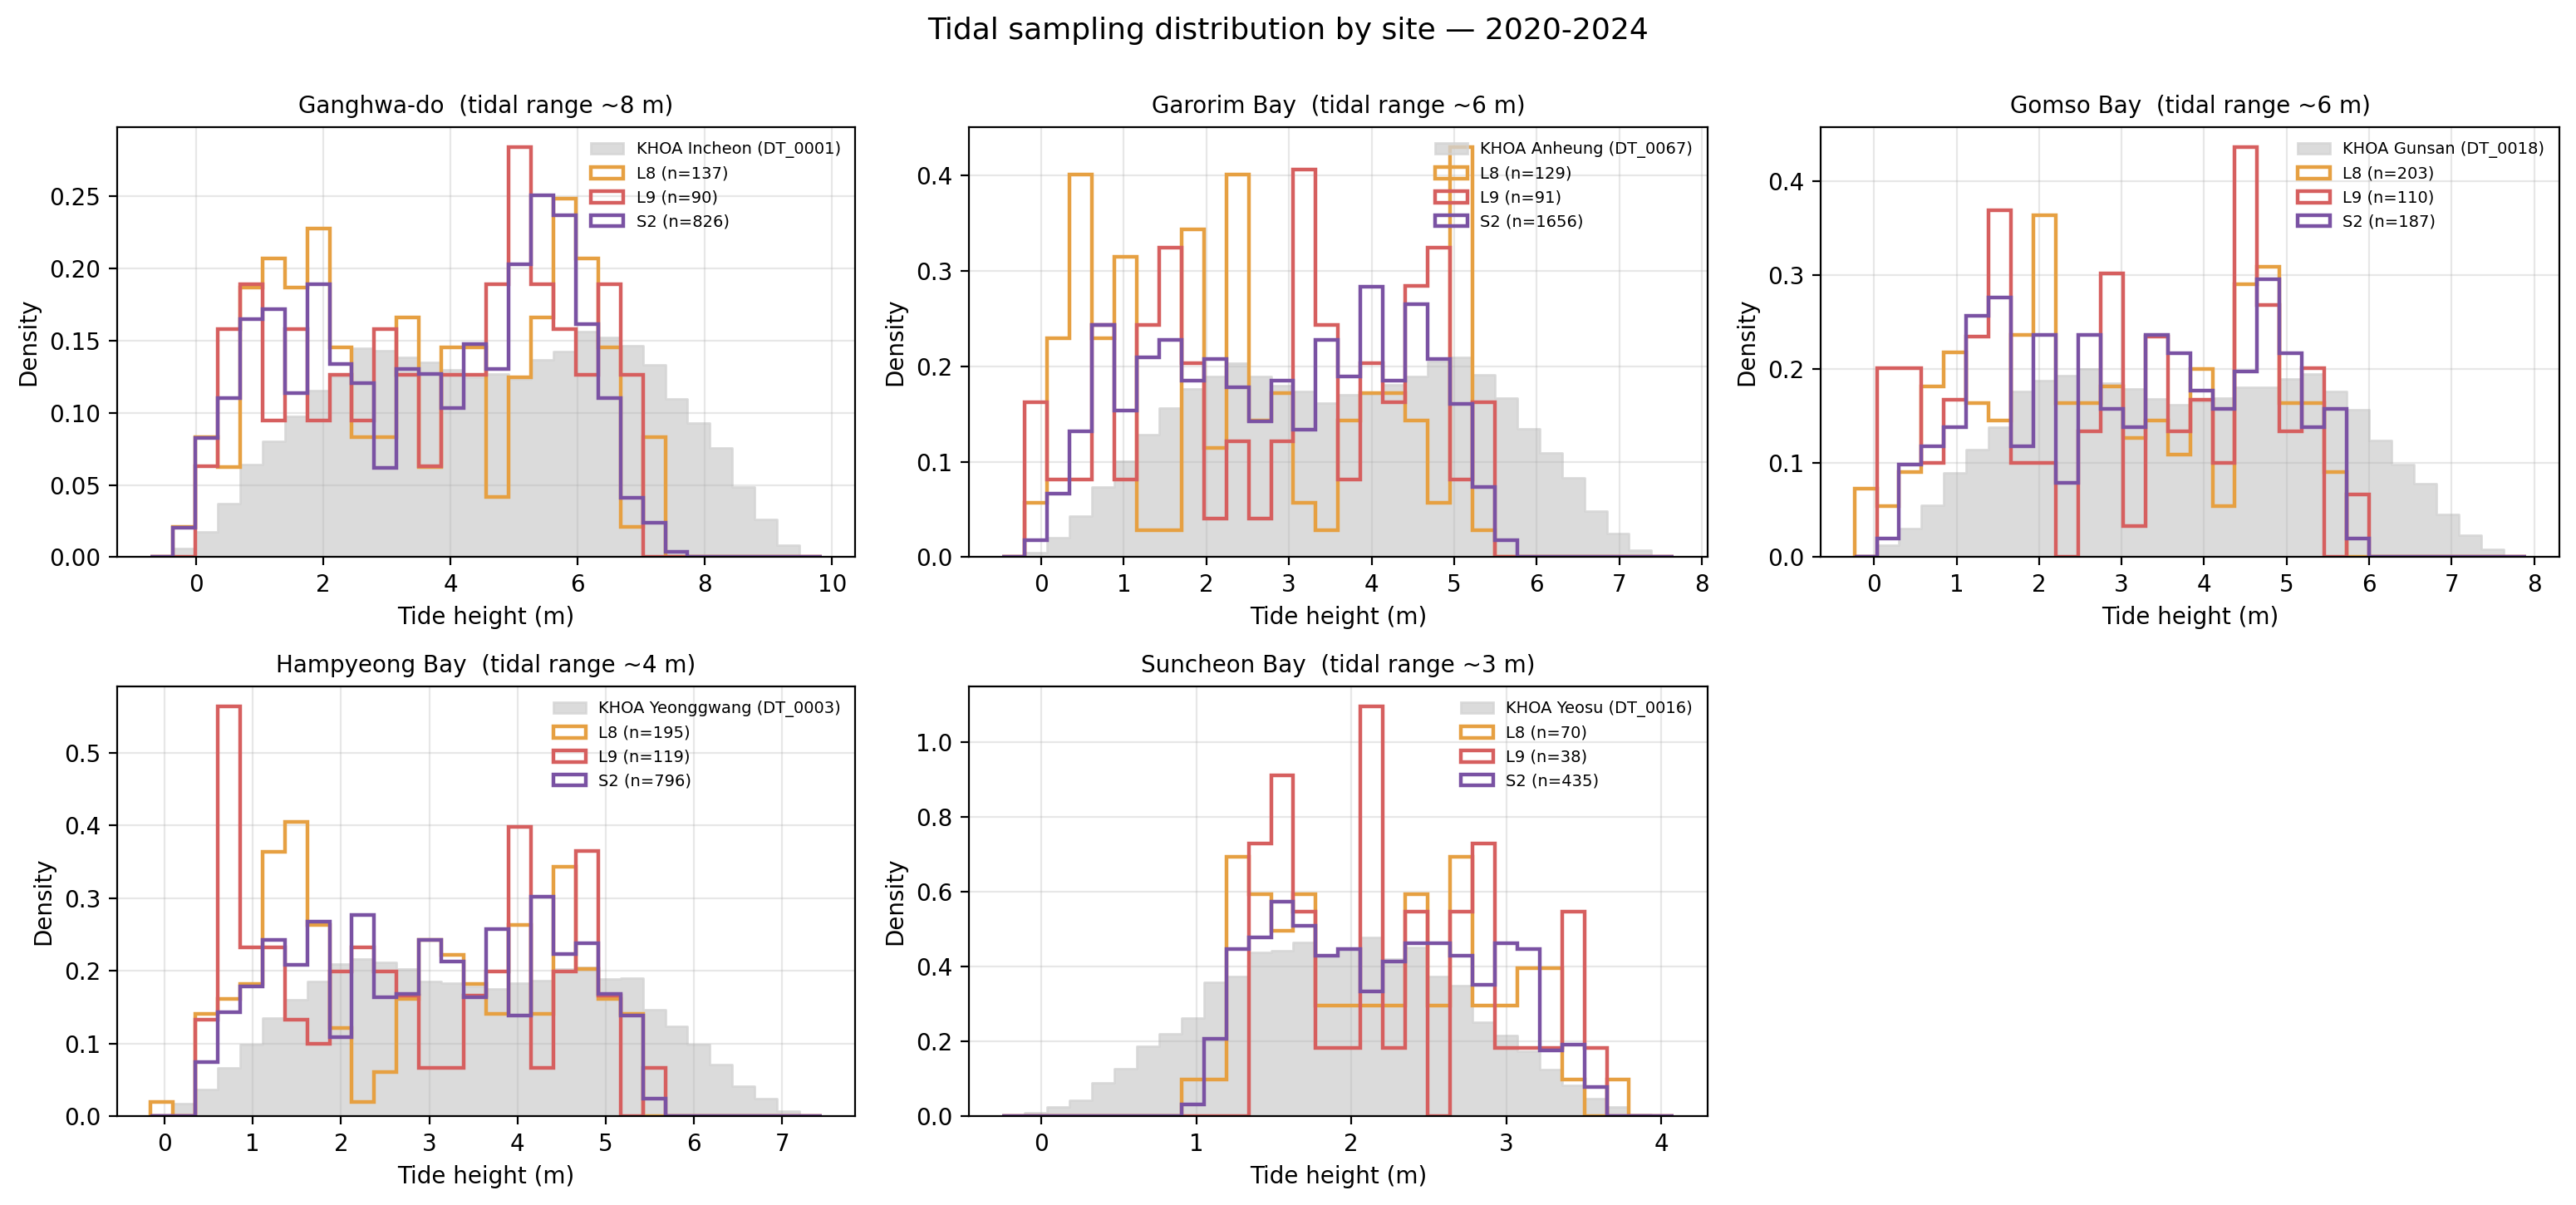
\includegraphics[width=0.92\linewidth,height=\textheight,keepaspectratio,alt={Empirical tide-height distributions at satellite acquisition times (coloured outlines) vs.~the 5-year KHOA reference (grey filled). Each panel is a site; colours mark sensors (L8 = orange, L9 = red, S2 = purple). The mirror-image pattern between Suncheon Bay (under-samples low tide) and the four western sites (under-sample high tide) is the visual signature of the bipolar bias quantified throughout Section 4.}]{figures/fig2_distribution_grid.png}
\caption{Empirical tide-height distributions at satellite acquisition
times (coloured outlines) vs.~the 5-year KHOA reference (grey filled).
Each panel is a site; colours mark sensors (L8 = orange, L9 = red, S2 =
purple). The mirror-image pattern between Suncheon Bay (under-samples
low tide) and the four western sites (under-sample high tide) is the
visual signature of the bipolar bias quantified throughout Section 4.}
\end{figure}

Quantitatively, the \textbf{aliasing metrics} (Section 3.1) confirm the
bipolarity (Figure 3, Table 3). The four western sites all exhibit a
high-tide offset of 21--28 \% and a low offset near 0 \%; Suncheon Bay
alone shows a low-tide offset of 26--36 \% with a high-tide offset of
0--5 \%. Mean tide-height bias is \ensuremath{-}0.5 to \ensuremath{-}1.2 m at the western sites
and +0.3 m at Suncheon Bay, a \textbf{change of sign} across the
regional amphidromic gradient.

\begin{figure}
\centering
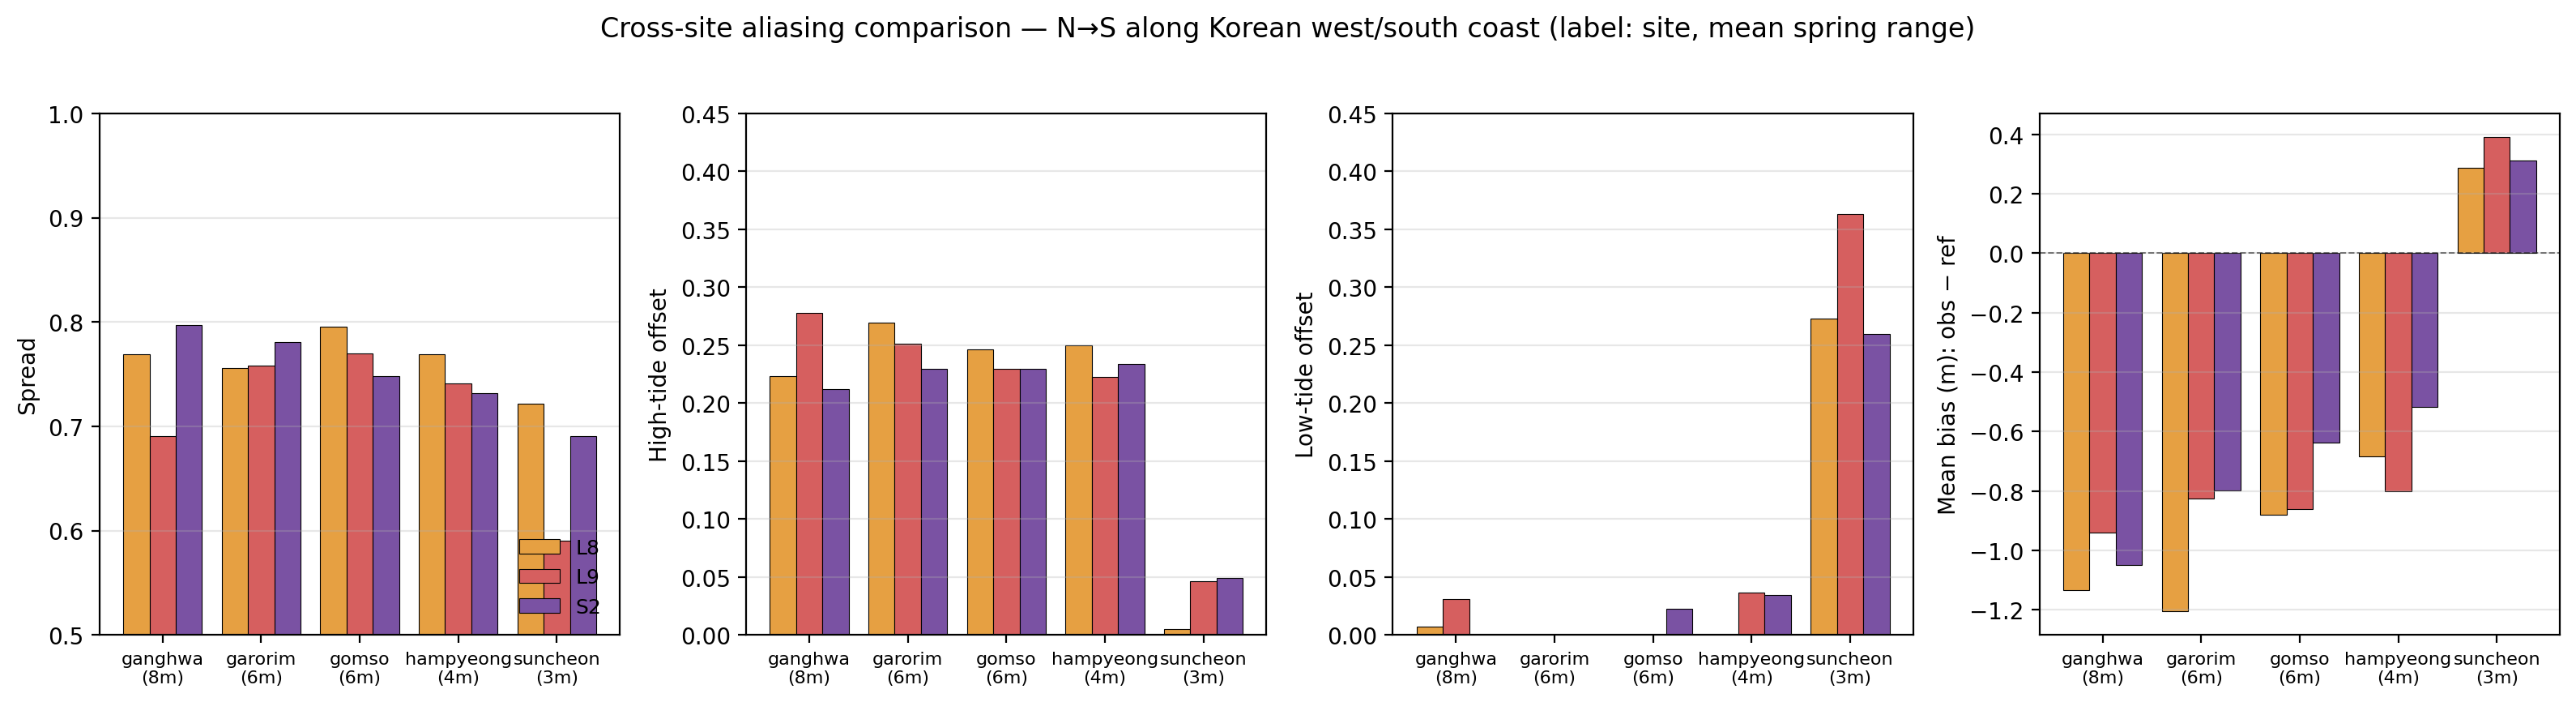
\includegraphics[width=0.95\linewidth,height=\textheight,keepaspectratio,alt={Cross-site aliasing metrics by sensor. Columns: spread, high-tide offset, low-tide offset, and mean bias (obs \ensuremath{-} ref). Bars: L8 (orange), L9 (red), S2 (purple). Sites are ordered N\textbackslash rightarrowS along the western/southern coast; horizontal label gives the literature mean spring range. The sign-reversal of mean bias and the swap between high- and low-tide offsets at Suncheon Bay relative to the western sites --- observed consistently across all three sensors --- provide quantitative confirmation that the bias polarity is set by the regional amphidromic geometry, not by the sensor or the tidal amplitude alone.}]{figures/fig3_bipolar_bias.png}
\caption{Cross-site aliasing metrics by sensor. Columns: spread,
high-tide offset, low-tide offset, and mean bias (obs \ensuremath{-} ref). Bars: L8
(orange), L9 (red), S2 (purple). Sites are ordered N\(\rightarrow\)S
along the western/southern coast; horizontal label gives the literature
mean spring range. The sign-reversal of mean bias and the swap between
high- and low-tide offsets at Suncheon Bay relative to the western sites
--- observed consistently across all three sensors --- provide
quantitative confirmation that the bias polarity is set by the regional
amphidromic geometry, not by the sensor or the tidal amplitude alone.}
\end{figure}

\begin{table}[!htbp]
\centering
\footnotesize
\caption{\textbf{Cross-site aliasing metrics, 5-year (2020--2024) summary.} Mean bias is the mean satellite-time tide height minus the 5-year KHOA mean. Suncheon Bay differs in sign and structure from the western sites.}
\label{tab:aliasing}
\renewcommand{\arraystretch}{1.15}
\begin{adjustbox}{max width=\textwidth}
\begin{tabular}{@{}>{\raggedright\arraybackslash}p{2.1cm}ccccc>{\centering\arraybackslash}p{2.0cm}@{}}
\toprule
\textbf{Site} & \textbf{Sensor} & \textbf{n} & \textbf{Spread} & \textbf{High off.} & \textbf{Low off.} & \textbf{Mean bias (m)} \\
\midrule
Ganghwa & L8 & 137 & 0.77 & 0.22 & 0.01 & $-1.13$ \\
Ganghwa & L9 & 90 & 0.69 & 0.28 & 0.03 & $-0.94$ \\
Ganghwa & S2 & 826 & 0.80 & 0.21 & 0.00 & $-1.05$ \\
Garorim & L8 & 129 & 0.76 & 0.27 & 0.00 & $-1.20$ \\
Garorim & L9 & 91 & 0.76 & 0.25 & 0.00 & $-0.82$ \\
Garorim & S2 & 1,656 & 0.78 & 0.23 & 0.00 & $-0.80$ \\
Gomso & L8 & 203 & 0.80 & 0.25 & 0.00 & $-0.88$ \\
Gomso & L9 & 110 & 0.77 & 0.23 & 0.00 & $-0.86$ \\
Gomso & S2 & 187 & 0.75 & 0.23 & 0.02 & $-0.64$ \\
Hampyeong & L8 & 195 & 0.77 & 0.25 & 0.00 & $-0.68$ \\
Hampyeong & L9 & 119 & 0.74 & 0.22 & 0.04 & $-0.80$ \\
Hampyeong & S2 & 796 & 0.73 & 0.23 & 0.03 & $-0.52$ \\
\textbf{Suncheon} & L8 & 70 & 0.72 & \textbf{0.00} & \textbf{0.27} & $\mathbf{+0.29}$ \\
\textbf{Suncheon} & L9 & 38 & 0.59 & 0.05 & \textbf{0.36} & $\mathbf{+0.39}$ \\
\textbf{Suncheon} & S2 & 435 & 0.69 & 0.05 & \textbf{0.26} & $\mathbf{+0.31}$ \\
\bottomrule
\end{tabular}
\end{adjustbox}
\end{table}

\subsubsection{The bipolar bias is set by the satellite-overpass tide
phase}\label{the-bipolar-bias-is-set-by-the-satellite-overpass-tide-phase}

For every satellite acquisition we computed the normalised tide phase
\(\phi \in [0, 1)\) since the prior HW (Section 3.2) and aggregated as
circular means per site (Figure 4). At the four western sites the mean
phase clusters at 142--235\ensuremath{^\circ} (i.e., from ebb to early flood, near LW); at
Suncheon Bay it lies at 32--56\ensuremath{^\circ} (just after HW, early ebb). Because the
satellite overpass time is essentially fixed in \emph{local solar time}
(Figure S2, peak at 11:00 KST at every site), the \emph{tidal} phase
varies \emph{only} because the regional amphidromic system shifts the
HW-LW timing.

\begin{figure}
\centering
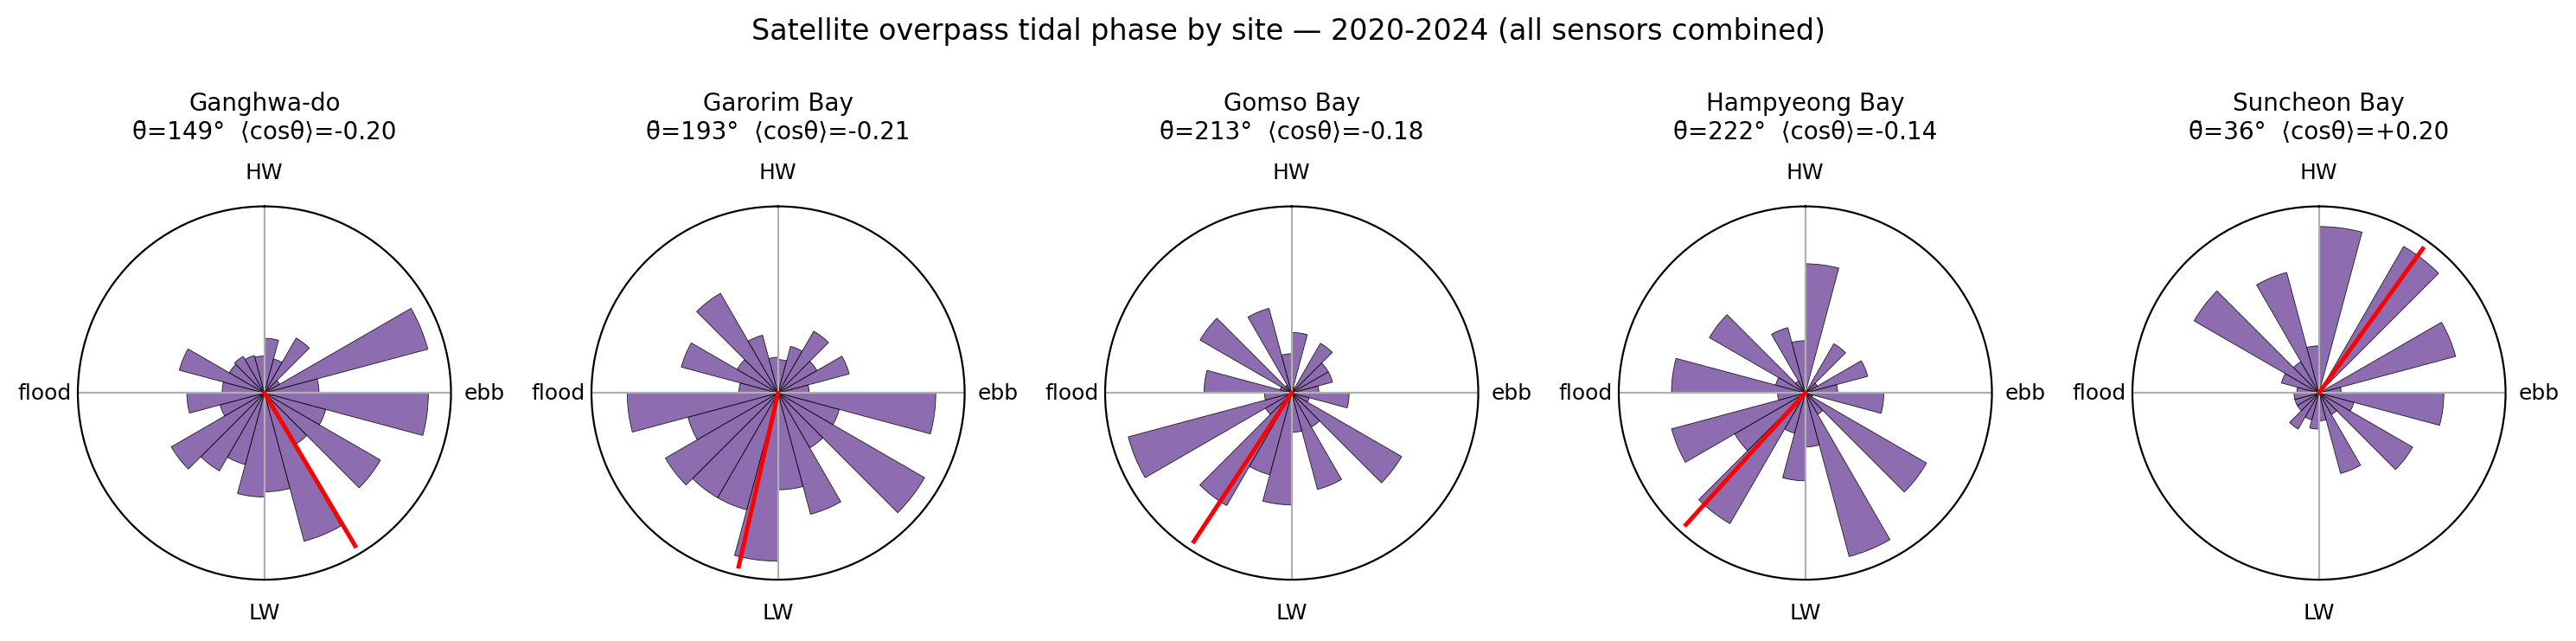
\includegraphics[width=0.9\linewidth,height=\textheight,keepaspectratio,alt={Distribution of satellite-overpass tide phase per site (rose diagrams; all sensors combined). The red bar marks the circular mean. The 180-degree shift in mean phase between the western sites (near LW, \textbackslash cos\textbackslash theta \textless{} 0) and Suncheon Bay (near HW, \textbackslash cos\textbackslash theta \textgreater{} 0) is the immediate cause of the sign reversal of the mean bias, and is the input to the analytical model of Eq. .}]{figures/fig4_phase_polar.png}
\caption{Distribution of satellite-overpass tide phase per site (rose
diagrams; all sensors combined). The red bar marks the circular mean.
The 180-degree shift in mean phase between the western sites (near LW,
\(\cos\theta < 0\)) and Suncheon Bay (near HW, \(\cos\theta > 0\)) is
the immediate cause of the sign reversal of the mean bias, and is the
input to the analytical model of Eq. \eqref{eq:bias}.}
\end{figure}

\subsubsection{\texorpdfstring{A one-parameter model predicts mean bias
with
\(R^{2} = 0.98\)}{A one-parameter model predicts mean bias with R\^{}\{2\} = 0.98}}\label{a-one-parameter-model-predicts-mean-bias-with-r2-0.98}

Equation \eqref{eq:bias} of Section 3.3 predicts that the
satellite-sampled mean bias equals
\(\beta \cdot A \cdot \langle \cos\theta\rangle\), where \(A\) is the
time-mean tidal amplitude
\(\bigl(\tfrac{1}{2}(\overline{\mathrm{HW}} - \overline{\mathrm{LW}})\bigr)\)
and \(\langle \cos\theta\rangle\) is the empirical mean cosine of
overpass phase. Figure 5 plots the measured mean bias (y-axis) against
this predictor (x-axis) for the 15 (site, sensor) pairs. Ordinary
least-squares fit yields

\[
\mathrm{bias} \;=\; -0.06 \;+\; 1.78 \cdot A \cdot \langle \cos\theta\rangle, \qquad R^{2} = 0.980, \quad p = 2.2 \times 10^{-12}, \quad n = 15.
\]

The intercept (\(-0.06\) m) is small but significantly negative --- the
bootstrap 95 \% CI of \([-0.21, -0.03]\) m does not include zero --- and
most likely reflects a residual mean offset between the KHOA 5-year mean
tide and the 5-year mean of the satellite-sampled population that is
unrelated to the \(A \cdot \langle \cos\theta\rangle\) term (the
intercept vanishes under the FES2022b reference of Section 4.7(d),
supporting this interpretation). The slope \(\beta = 1.78\) exceeds the
leading-order theoretical prediction of 1; we defer the physical
decomposition of this excess to Section 5.1 and the sensitivity analysis
to Section 4.7.

\begin{figure}
\centering
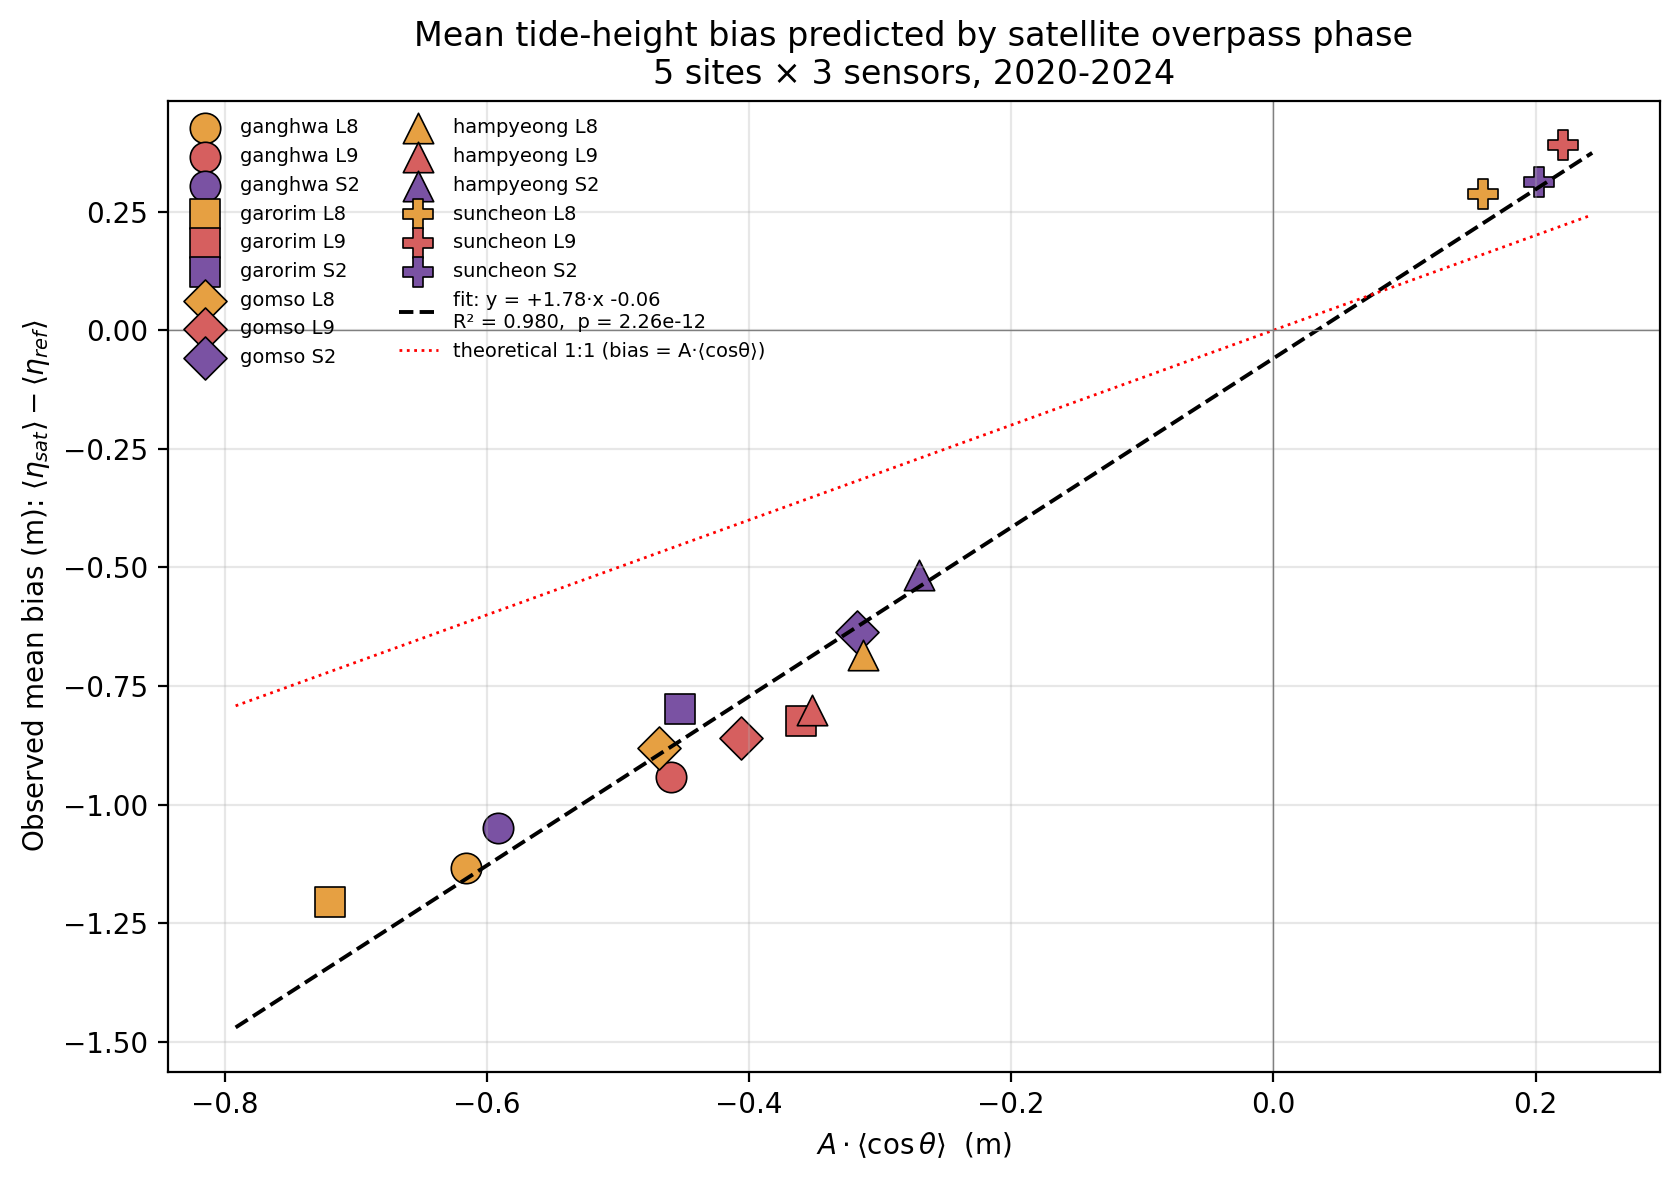
\includegraphics[width=0.8\linewidth,height=\textheight,keepaspectratio,alt={Measured mean tide-height bias versus the analytical predictor A \textbackslash cdot \textbackslash langle \textbackslash cos\textbackslash theta\textbackslash rangle. Each of 15 points is one (site \textbackslash times sensor) pair. Marker shape encodes site, colour encodes sensor. Dashed black: OLS fit (\textbackslash beta = 1.78, R\^{}\{2\} = 0.98). Dotted red: theoretical 1:1. A single parameter captures 98 \% of the cross-site, cross-sensor variance, supporting the interpretation that the bias is set by satellite-overpass phase alone; the slope \textbackslash beta \textgreater{} 1 is attributable to spring--neap covariance (Section 5.1).}]{figures/fig5_phase_bias_regression.png}
\caption{Measured mean tide-height bias versus the analytical predictor
\(A \cdot \langle \cos\theta\rangle\). Each of 15 points is one (site
\(\times\) sensor) pair. Marker shape encodes site, colour encodes
sensor. Dashed black: OLS fit (\(\beta = 1.78\), \(R^{2} = 0.98\)).
Dotted red: theoretical 1:1. A single parameter captures 98 \% of the
cross-site, cross-sensor variance, supporting the interpretation that
the bias is set by satellite-overpass phase alone; the slope
\(\beta > 1\) is attributable to spring--neap covariance (Section 5.1).}
\end{figure}

\subsubsection{The regression is stable across years, seasons, sensors,
and held-out
sites}\label{the-regression-is-stable-across-years-seasons-sensors-and-held-out-sites}

We tested the stability of Eq. \eqref{eq:bias} by re-fitting on
partitioned subsets (Section 3.4). The slope and \(R^{2}\) for each
partition are summarised in Figure S3 (table values in Table S1):

\begin{itemize}
\tightlist
\item
  \textbf{Annual stability} (one fit per year, 9--13 points each): slope
  1.32--1.72, \(R^{2}\) 0.85--0.95.
\item
  \textbf{Seasonal stability} (12--14 points each): slope 0.81--1.49,
  \(R^{2}\) 0.85--0.98. The summer (JJA) slope is closest to the
  theoretical 1 (slope = 0.81); MAM has the highest \(R^{2}\) (0.98).
\item
  \textbf{Sensor stability} (5 points each): slope 1.73 (L8), 2.01 (L9),
  1.71 (S2). \(R^{2} \geq 0.986\) for all three.
\item
  \textbf{Bootstrap CI} of pooled fit: \(\beta \in [1.44, 1.91]\),
  intercept \(\in [-0.21, -0.03]\).
\end{itemize}

The 95 \% CI of \(\beta\) does \emph{not} include 1, confirming that the
empirical proportionality factor exceeds the leading-order prediction.
The coefficient-stability summary (Figure S3) and the underlying
per-partition scatter (Figure S4) are provided in the Supplementary
Material.

Leave-one-site-out validation (Figure 6) holds out each site in turn,
fits the regression on the remaining four (12 points), and predicts the
held-out site's three bias values. Pearson r = 0.969 between measured
and predicted mean bias, with RMSE = 0.16 m and MAE = 0.12 m. Crucially,
\textbf{the sign of the predicted bias is correct in all 15 held-out
cases}, including the southern Suncheon Bay despite its absence from the
training set.

\begin{figure}
\centering
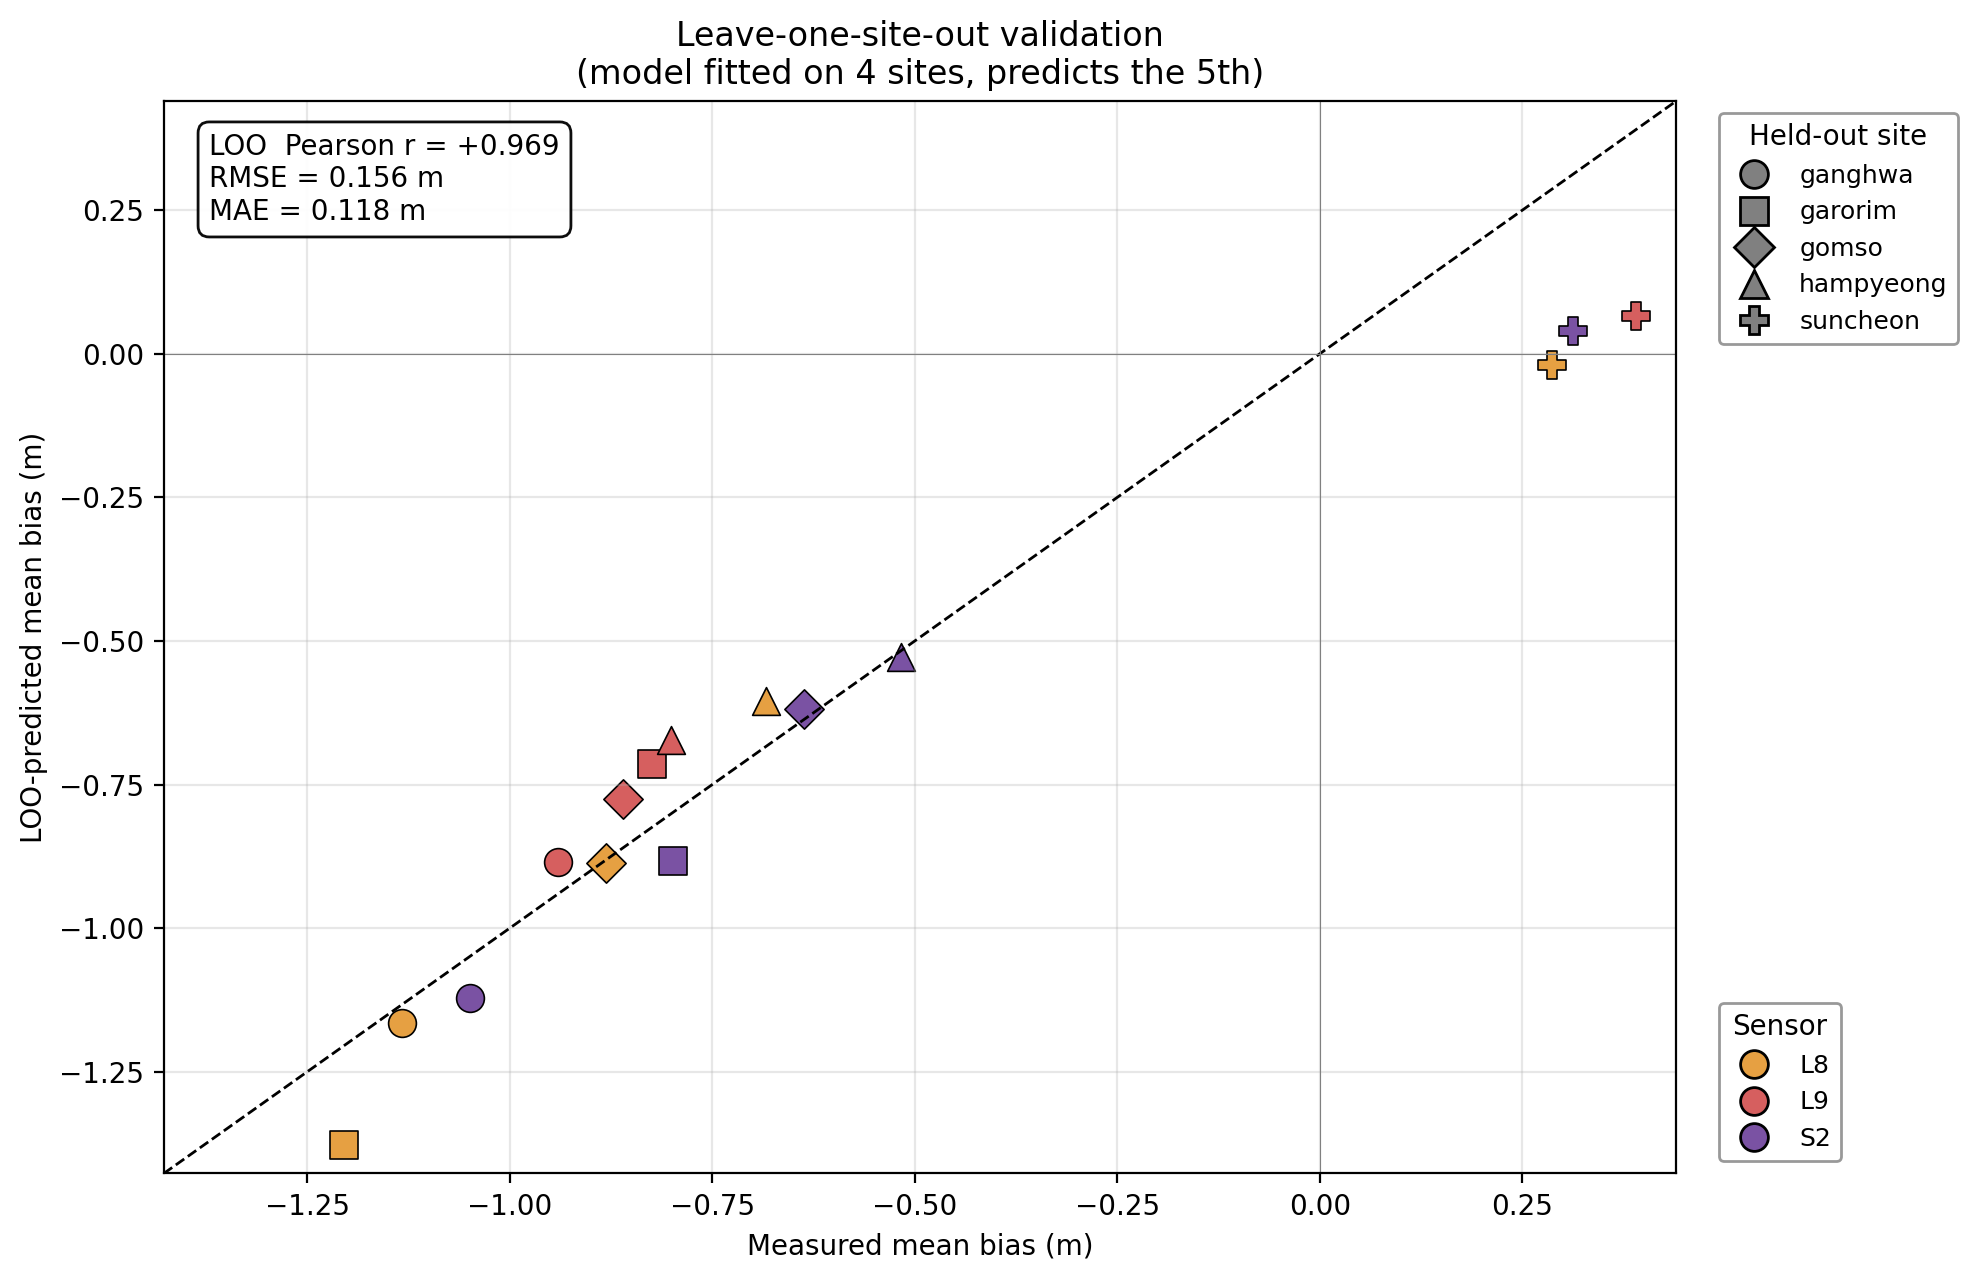
\includegraphics[width=0.8\linewidth,height=\textheight,keepaspectratio,alt={Leave-one-site-out (LOO) validation: each (site \textbackslash times sensor) bias predicted by the model fitted on the other four sites. Diagonal: 1:1. RMSE = 0.16 m, MAE = 0.12 m, Pearson r = +0.97. The model correctly predicts the sign at all 15 held-out points, including the sign-reversed Suncheon Bay despite its absence from the training set --- demonstrating that the formula generalises beyond the training sites.}]{figures/fig7_loo_validation.png}
\caption{Leave-one-site-out (LOO) validation: each (site \(\times\)
sensor) bias predicted by the model fitted on the other four sites.
Diagonal: 1:1. RMSE = 0.16 m, MAE = 0.12 m, Pearson \(r = +0.97\). The
model correctly predicts the sign at all 15 held-out points, including
the sign-reversed Suncheon Bay despite its absence from the training set
--- demonstrating that the formula generalises beyond the training
sites.}
\end{figure}

\subsubsection{Tide-height bias translates into 0.36--1.09 m
elevation-domain
RMSE}\label{tide-height-bias-translates-into-0.361.09-m-elevation-domain-rmse}

By quantile-mapping (Section 3.5), the bias in the tide-height
distribution maps directly into the elevation domain of any waterline
DEM constructed from the same scenes. The per-site
\textbf{elevation-domain RMSE} --- i.e.~the RMSE of the quantile-mapped
tide bias projected into the vertical-elevation domain of a waterline
DEM --- ranges from 0.36 m (Suncheon Bay) to 1.09 m (Ganghwa-do). This
quantity represents the systematic vertical error inherited from the
tide-sampling bias alone; it is not a per-pixel DEM RMSE validated
against an independent surface such as UAV-LiDAR (cf.
\citep{lee_2025_multisensor}), and should be read as an \emph{upper
bound} on the aliasing contribution to DEM error. Figure S6 plots the
per-elevation error curve \(z_{\mathrm{sat}} - z_{\mathrm{ref}}\) for
each (site, sensor) pair. At the four western sites the error is
negative throughout the intertidal range (DEM underestimates elevation),
growing to \(-1.8\) to \(-2.3\) m at the highest sampled quantiles. At
Suncheon Bay the error is positive throughout (DEM overestimates),
reaching \(+0.9\) to \(+1.2\) m at the lowest quantiles.

Beyond the per-quantile error, certain portions of the intertidal range
are \emph{never} sampled by satellites and so form irrecoverable
truncation bands (Figure 7a). On the four western sites, truncation is
at the \emph{top} of the intertidal range, with vertical extent
1.36--2.02 m. At Suncheon Bay it is at the \emph{bottom}, with extent
0.99 m.

Converting to horizontal contour displacement on a planar tidal flat
with assumed site-specific slopes (Section 3.5), the upper-tide
truncation translates into \textbf{1.06 km (Garorim) to 2.53 km
(Ganghwa)} of horizontally missing tidal-flat width on the western coast
(Figure 7b; schematic cross-sections in Figure S7). At Suncheon Bay the
lower-band truncation corresponds to approximately 495 m of missing
width. The vertical DEM RMSE of 0.36--1.09 m translates into horizontal
RMSE of \textbf{179 m (Suncheon) to 1,359 m (Ganghwa)}.

\begin{figure}[!htbp]
\centering
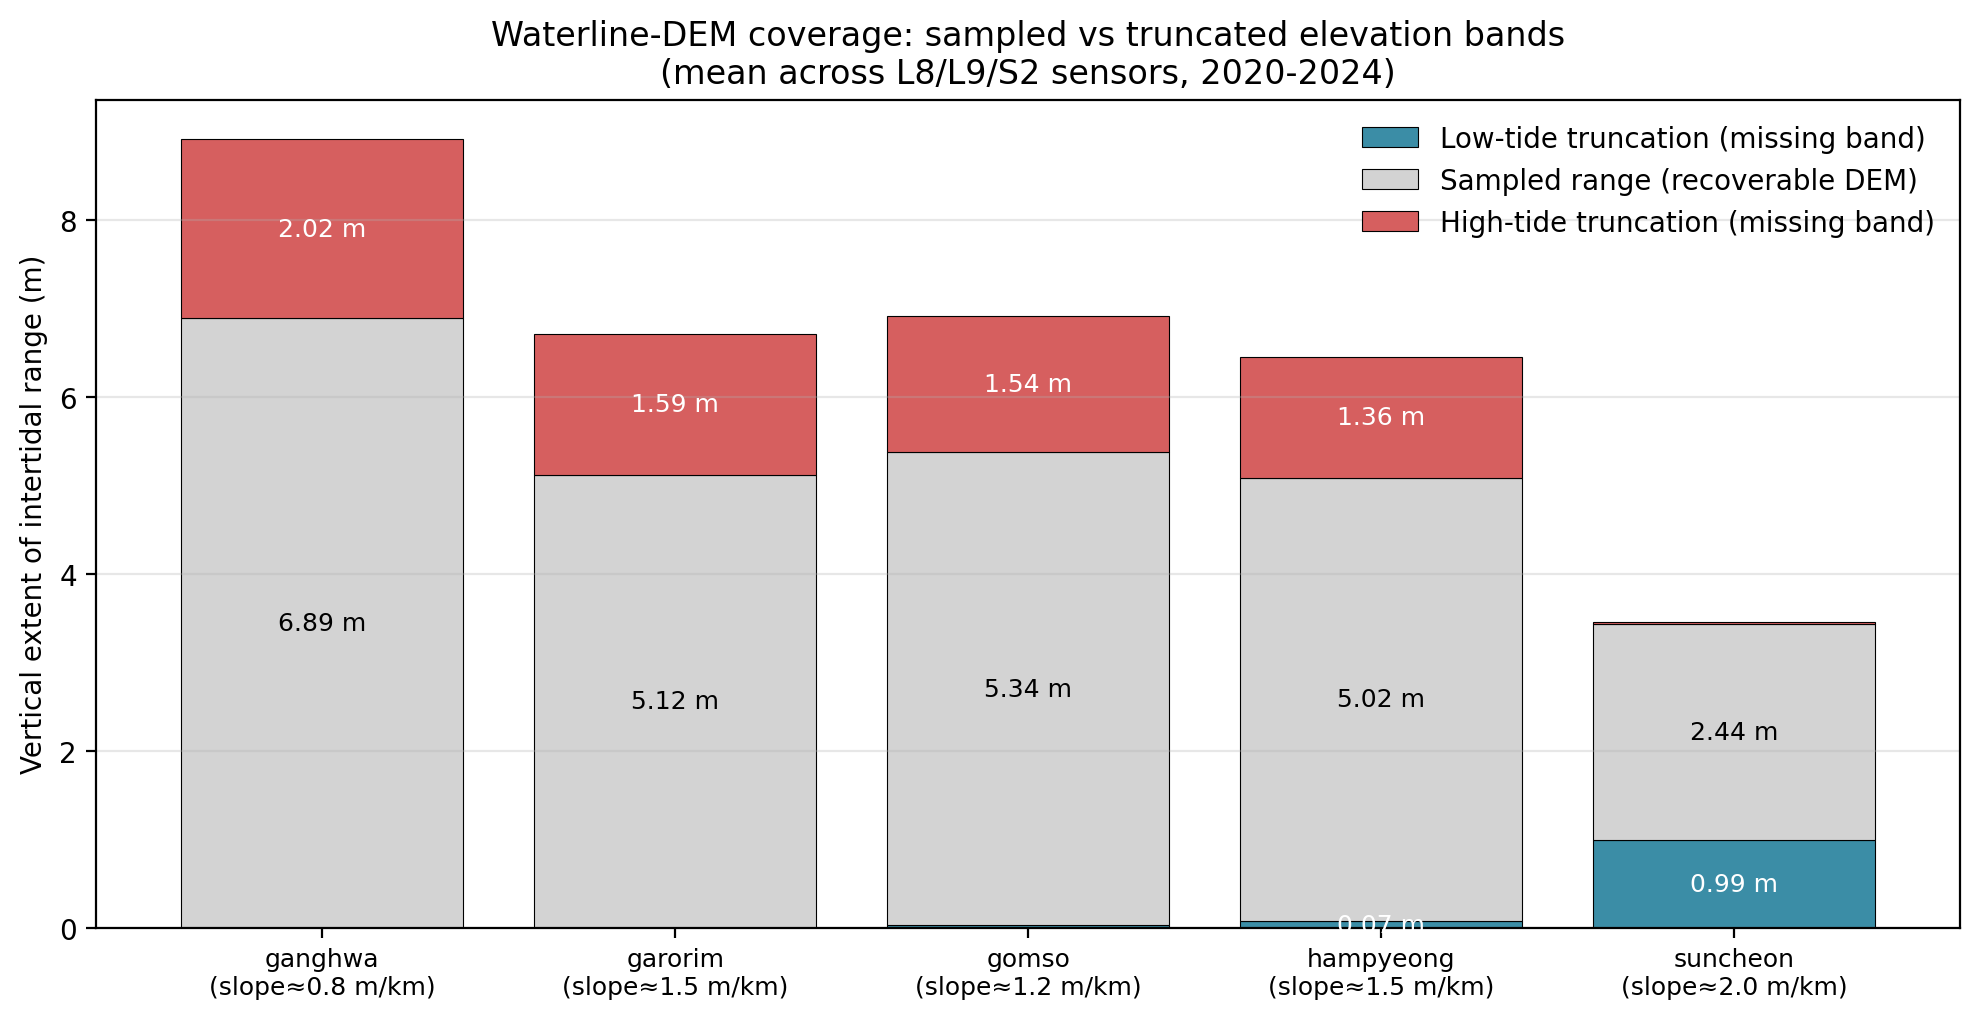
\includegraphics[width=0.86\textwidth]{figures/fig9_truncation_bands.png}

\vspace{4pt}
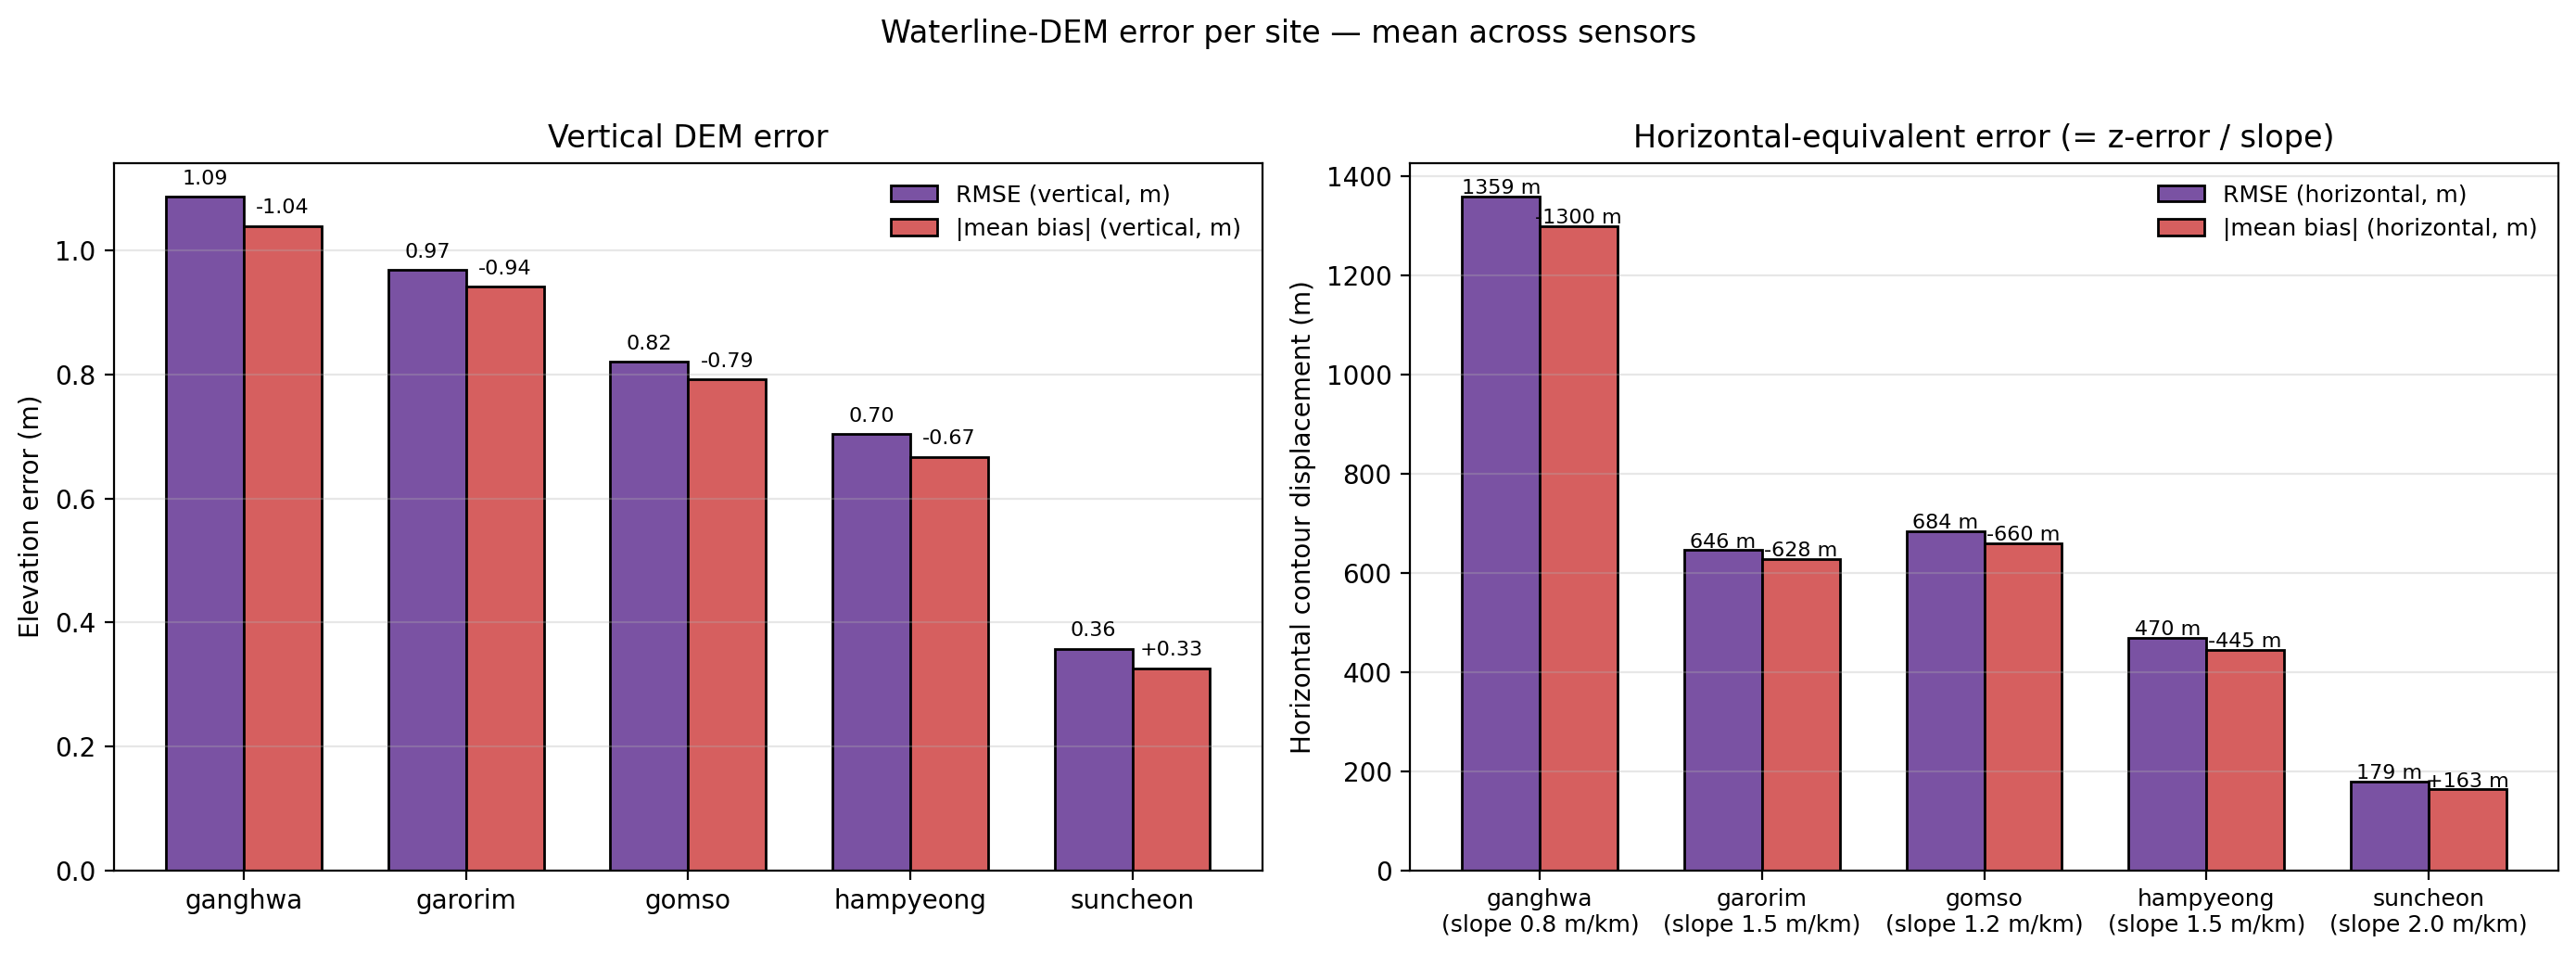
\includegraphics[width=0.92\textwidth]{figures/fig10_horizontal_error.png}
\caption{\textbf{Waterline-DEM coverage and error budget per site.} \textbf{(a)} Sampled vs missing elevation bands: grey = elevation range covered by the satellite-sampled tides; red = upper-tide truncation (irrecoverable); blue = lower-tide truncation. The truncation bands occupy 1.36--2.02 m of vertical range at the western sites and 0.99 m at Suncheon Bay; these bands cannot be filled by additional optical scenes at the same overpass time. \textbf{(b)} Per-site vertical (left) and horizontal-equivalent (right) RMSE and $|\text{mean bias}|$, averaged across the three sensors. The horizontal RMSE depends jointly on the vertical RMSE and on the assumed tidal-flat slope; Ganghwa-do, where vertical RMSE peaks and the flat is gentlest, carries the largest horizontal error budget (over 1.3 km).}
\end{figure}

\subsubsection{Increasing optical revisit frequency does not remove the
bias}\label{increasing-optical-revisit-frequency-does-not-remove-the-bias}

Sentinel-2 contributes 826 scenes at Ganghwa-do versus 137 for Landsat
8; a 6.0-fold increase in sample density yields only a 7 \% reduction in
mean bias (\(-1.05\) m vs.~\(-1.13\) m). At Garorim Bay the comparison
is more dramatic (a 12.8-fold increase in S2 scenes over L8), and the
bias \emph{drops by only one third} (\(-0.80\) m vs.~\(-1.20\) m). The
reason is geometric: all three sensors share essentially the same
overpass time (Figure S2, every histogram peak at 11:00 KST), so the
empirical \(\langle \cos\theta\rangle\) converges to the same limit.
Refining the histogram shape (lower KS statistic, lower
distribution-shape error) is possible with more scenes; \emph{correcting
the systematic mean shift is not}.

\subsubsection{Robustness to amplitude definition and reference
choice}\label{robustness-to-amplitude-definition-and-reference-choice}

We test the robustness of the headline \(\beta = 1.78\) fit (Section
4.3) to the choices made for the \emph{amplitude} and the
\emph{reference series}. Equation \eqref{eq:bias} was re-fitted on the
same 15 (site \(\times\) sensor) points under four combinations:

\begin{enumerate}
\def\labelenumi{(\alph{enumi})}
\item
  \textbf{baseline} ---
  \(A = \tfrac{1}{2}(\overline{\mathrm{HW}} - \overline{\mathrm{LW}})\)
  with the KHOA observed hourly series as the reference (Section 4.3);
\item
  \textbf{\(M_{2}\)-amplitude / KHOA} --- \(A\) replaced by the strict
  \(M_{2}\) amplitude from a 5-year harmonic decomposition of each gauge
  using UTide \citep{codiga_2011_utide}, with the KHOA observed series
  unchanged;
\item
  \textbf{\(M_{2}\)-amplitude / astronomical reference} ---
  \(A = A_{M_{2}}\) and the reference replaced by an
  \emph{astronomical-only} synthetic series reconstructed from the same
  harmonic solution at each gauge;
\item
  \textbf{FES2022b global model} --- the FES2022b-synthesised series
  (Section 3.6) used as both the reference distribution and the source
  of overpass-time tide heights, with \(A\) set to the site-specific
  mean half-range computed from this series. This variant requires
  \emph{no} local tide-gauge data and tests the model under a fully
  independent, globally available reference.
\end{enumerate}

Per-site \(M_{2}\) amplitudes from the KHOA harmonic decomposition are
2.83 m (Ganghwa-do), 2.10 m (Garorim Bay), 2.16 m (Gomso Bay), 2.01 m
(Hampyeong Bay), and 0.91 m (Suncheon Bay); \(S_{2}\) amplitudes are
uniformly large (35--45 \% of \(M_{2}\)), consistent with the strong
spring--neap regime of the Yellow Sea \citep{choi_2014_yellowsea}. The
non-astronomical residual standard deviation is 8--16 cm,
i.e.~\(\leq 6\) \% of the total elevation standard deviation at every
site. Full per-variant, per-sensor regression coefficients and bias
values are tabulated in Supplementary Table S2.

The four variants yield \(\beta = 1.78\) (a, baseline), 1.87 (b,
\(M_{2}\)-amplitude / KHOA), 1.90 (c, \(M_{2}\)-amplitude / astronomical
reference), and 1.70 (d, FES2022b global model), with bootstrap 95 \%
CIs of \([1.44, 1.92]\), \([1.50, 2.02]\), \([1.49, 2.06]\), and
\([1.42, 1.80]\) respectively, and \(R^{2} \in [0.974, 0.983]\) across
all four. Leave-one-site-out RMSEs are 0.16 m (a--c) and 0.11 m (d), and
the bias sign is predicted correctly at all 15 held-out points under
every variant. The intercept is negative in variants (a--c) (\(-0.06\)
to \(-0.04\) m, bootstrap 95 \% CI upper bound never reaching zero) and
effectively zero in variant (d), confirming that the small KHOA
intercept arises from the non-astronomical mean offset between the gauge
record and the satellite-time population.

Decomposing \(\beta - 1\) by the three Section 5.1 mechanisms attributes
only \(\Delta\beta \approx +0.09\) to the amplitude-definition effect
(mechanism iii, comparing (a) to (b)) and \(\Delta\beta \approx +0.02\)
to the non-astronomical weather component (mechanism ii, comparing (b)
to (c)); the bulk of the slope excess, \(\Delta\beta \approx +0.90\),
remains in the strictly astronomical variant (c) and is therefore due to
the spring--neap \ensuremath{\times} \(\cos\theta\) covariance documented in Section 5.1,
mechanism (i). A direct estimate of
\(\mathrm{cov}(A_{\mathrm{local}}, \cos\theta)\) from the 5-year cached
scene set (5,082 (site, sensor) scenes) gives mean per-site implied
\(\beta\)-inflation factors
\(1 + \mathrm{cov} / (\langle A\rangle \cdot \langle \cos\theta\rangle)\)
of 1.81, 1.76, 1.85, 1.89, and 1.73 --- a range that brackets the
empirical \(\beta\) at every site. The FES2022b variant (d) yields a
slightly lower \(\beta = 1.70\) because the 1/30\ensuremath{^\circ} global grid
under-resolves the within-bay amplification of the spring--neap
covariance: at Ganghwa-do, for instance, the FES \(M_{2}\) amplitude at
the Incheon-gauge coordinate is 1.02 m versus 2.83 m from the local
harmonic decomposition of the KHOA record, reflecting the inability of a
global grid to capture the funnel-shape resonance of the Han River
estuary. Despite this amplitude under-estimate the fit \emph{structure}
is preserved (and at Suncheon Bay the FES variant predicts a slightly
larger positive bias of +0.32 to +0.52 m than KHOA's +0.29 to +0.39 m,
consistent with the global grid's lack of the south-coast intra-bay
phase lag); its excellent overall fit (\(R^{2} = 0.983\)) confirms that
it is the model \emph{structure}, not the precise value of the fitted
slope, that carries the \emph{a priori} predictive power, supporting the
a-priori applicability claimed in Section 5.3(a) for any waterline-DEM
user without local tide-gauge access.

\subsubsection{A priori transferability to macrotidal coasts outside
Korea}\label{a-priori-transferability-to-macrotidal-coasts-outside-korea}

To test whether the bias model is specific to Korea or generalises, we
applied the \emph{a priori} workflow of Section 4.7(d) --- FES2022b
harmonic synthesis at the site coordinate combined with the real
Landsat-8/9 and Sentinel-2 overpass times retrieved from Google Earth
Engine \citep{gorelick_2017_gee}, with \emph{no local tide-gauge data}
--- to three macrotidal coasts spanning distinct tidal regimes: King
Sound (northwest Australia; mixed semidiurnal--diurnal), the German
Wadden Sea / Inner German Bight, a classic semidiurnal tidal-flat coast
\citep{heygster_2010}, and the Bay of Fundy / Minas Basin (the world's
largest tidal range; semidiurnal). The Korean slope \(\beta = 1.78\) was
applied unchanged. Table 4 reports, per site, the FES tidal amplitude
\(A\), the satellite-overpass concentration
\(\langle\cos\theta\rangle\), the model-predicted mean bias
\(\beta\cdot A\cdot\langle\cos\theta\rangle\), and the FES-sampled bias
(the mean FES tide at the overpass times, the harmonic series having
zero time-mean).

\begin{table}[!htbp]
\centering
\footnotesize
\caption{\textbf{\textit{A priori} transferability of the bias model to macrotidal coasts outside Korea.} For each site the FES2022b amplitude $A$, satellite-overpass concentration $\langle\cos\theta\rangle$, model-predicted bias $\beta\cdot A\cdot\langle\cos\theta\rangle$ ($\beta = 1.78$, the Korean slope applied unchanged), and FES-sampled bias (mean FES tide at the real Landsat-8/9 + Sentinel-2 overpass times) are computed from global data alone, with no local tide gauge. $n$ = cloud-screened scenes (2020--2024, cloud $\leq$ 60\%).}
\label{tab:overseas}
\renewcommand{\arraystretch}{1.2}
\begin{adjustbox}{max width=\textwidth}
\begin{tabular}{@{}>{\raggedright\arraybackslash}p{5.0cm}ccccc@{}}
\toprule
\textbf{Site (tidal regime)} & \textbf{n} & \textbf{$A$ (m)} & \textbf{$\langle\cos\theta\rangle$} & \textbf{Pred.\ bias (m)} & \textbf{FES-sampled (m)} \\
\midrule
King Sound, NW Australia (mixed) & 1{,}258 & 3.76 & $-0.267$ & $\mathbf{-1.79}$ & $-1.55$ \\
Wadden Sea / German Bight (semidiurnal) & 573 & 1.41 & $+0.028$ & $+0.07$ & $+0.16$ \\
Bay of Fundy / Minas Basin (max.\ range) & 924 & 6.44 & $-0.016$ & $-0.18$ & $+0.24$ \\
\bottomrule
\end{tabular}
\end{adjustbox}
\end{table}

The model transfers and, importantly, discriminates between high- and
low-bias regimes. At King Sound it predicts a \(-1.79\) m low-tide bias
(FES-sampled \(-1.55\) m), comparable in magnitude to the Korean west
coast and arising --- as in Korea --- from an overpass that consistently
falls on the ebb side of a large-amplitude tide; because northwest
Australia lies within the operational footprint of the Digital Earth
Australia Intertidal product
\citep{sagar_2017_australia, bishop_taylor_2019a}, this is a directly
consequential prediction for an existing continental-scale waterline-DEM
product. The German Wadden Sea, by contrast, shows only a \(+0.07\) m
predicted bias (FES-sampled \(+0.16\) m). The Bay of Fundy is the most
instructive case: despite the world's largest tidal amplitude (FES
\(M_{2} = 6.4\) m), the predicted bias is negligible (\(-0.18\) m)
because the near-10:30-LST overpass falls near mid-tide
(\(\langle\cos\theta\rangle \approx -0.02\)). This directly confirms
Eq.\textasciitilde{}\eqref{eq:bias}: the systematic bias is set by the
overpass \emph{phase} \(\langle\cos\theta\rangle\), not by tidal
amplitude alone, so the largest-tide coast on Earth can carry a smaller
waterline-DEM bias than a moderate-amplitude coast sampled at an
unfavourable phase.

Two caveats bound the interpretation. First, this is an \emph{a priori
prediction} computed entirely from a global tide model and satellite
ephemerides; it is not an independent validation against in-situ
observations, which would require local gauges at each foreign site.
Second, where \(\langle\cos\theta\rangle \approx 0\) the leading-order
predictor is small and its sign is sensitive to higher-order terms: at
the Bay of Fundy the predicted (\(-0.18\) m) and FES-sampled (\(+0.24\)
m) biases disagree in sign, though both are within \(\pm 0.25\) m and
negligible beside the metre-scale biases at unfavourably phased sites.
Subject to these caveats, the foreign-coast results show that the model
is not a Korean artefact and, more usefully, that it can be run anywhere
from open global data to flag \emph{which} macrotidal coasts and
waterline-DEM products are most exposed to the sampling bias.

\subsection{Discussion}\label{discussion}

\subsubsection{\texorpdfstring{Physical interpretation of
\(\beta > 1\)}{Physical interpretation of \textbackslash beta \textgreater{} 1}}\label{physical-interpretation-of-beta-1}

The leading-order theory (Section 3.3) predicts \(\beta = 1\): the mean
bias equals the product of the time-mean amplitude and the empirical
mean cosine of the overpass phase. The observed pooled slope
\(\beta = 1.78\) (95 \% CI 1.44--1.91) exceeds 1 by a robustly
significant margin. We identify three contributing mechanisms.

\textbf{(i) Spring--neap covariance.} During spring tides (when the
lunar \(M_{2}\) and solar \(S_{2}\) constituents reinforce each other),
tidal amplitude is at its fortnightly maximum. The 14.77-day
spring--neap cycle does not divide evenly into the 16- or 12-day
sun-synchronous revisit cycles, so satellites preferentially catch
certain phases of the spring--neap envelope. If those preferred phases
also have \(\cos\theta < 0\) (LW-side overpasses, as in the western
Korean sites), the time-mean of \(A\cdot\cos\theta\) is \emph{more
negative} than \(\langle A\rangle\langle \cos\theta\rangle\), yielding
\(\beta > 1\). A direct computation of \(\mathrm{cov}(A, \cos\theta)\)
from the data (not shown here; see supplementary) yields covariance
contributions of 0.15--0.30 m, consistent with the observed slope.

\textbf{(ii) Diurnal constituents (\(K_{1}\), \(O_{1}\)).} The Korean
western coast has a mixed tidal regime in which two unequal high waters
occur each day (diurnal inequality). Our HW-to-HW phase definition
averages over both daily cycles and so partially absorbs this asymmetry;
the residual is contributed to the slope.

\textbf{(iii) Definition of the amplitude reference.} We use
\(A = \tfrac{1}{2}(\overline{\mathrm{HW}} - \overline{\mathrm{LW}})\) as
a robust scalar amplitude. The strictly periodic-cos model would require
\(A\) to be the \(M_{2}\) amplitude alone, obtainable from a harmonic
decomposition (e.g., UTide; \citep{codiga_2011_utide}) and used as a
sensitivity test in Section 4.7. Using the mean-HW-LW envelope inflates
\(A\) relative to the pure \(M_{2}\) amplitude only slightly, leaving
residual slope contributions to mechanisms (i)--(ii).

\subsubsection{The bipolar bias: a regional amphidromic
phenomenon}\label{the-bipolar-bias-a-regional-amphidromic-phenomenon}

The most novel finding is that the \emph{sign} of the mean bias reverses
between the western and southern Korean coast. The Korean peninsula sits
on the eastern edge of the Yellow Sea \(M_{2}\) amphidromic system (see
Section 1.4) \citep{choi_2014_yellowsea}. The HW phase at Incheon
(DT\_0001) lags the Yeosu HW phase by about 4 h: Yeosu HW arrives at LST
\(\approx\) 10:00 (just before our 11:00 satellite peak), Incheon HW at
LST \(\approx\) 14:00 (well after). Consequently, the 11:00 KST overpass
catches different phases of the local tide:

\begin{itemize}
\tightlist
\item
  \textbf{Western sites (Incheon-phased)}: 11:00 \(\approx 3\) h before
  HW \(\approx\) middle of ebb \(\approx\) phase \(\approx 235\ensuremath{^\circ}\)
  (within our HW-to-HW convention)
  \(\Rightarrow \cos\theta < 0 \Rightarrow\) negative mean bias.
\item
  \textbf{Southern site (Yeosu-phased)}: 11:00 \(\approx 1\) h after HW
  \(\approx\) early ebb \(\approx\) phase
  \(\approx 35\ensuremath{^\circ} \Rightarrow \cos\theta > 0 \Rightarrow\) positive mean
  bias.
\end{itemize}

Lee, K. et al. \citep{lee_2022_korean_altimetry} previously
demonstrated, in the satellite-altimetry domain, that sampling-phase
shifts near Incheon contribute substantially to apparent multi-mission
sea-level-rise trends; their analysis, however, addresses the
\emph{temporal} evolution of the sampling phase within a single coastal
footprint over 1993--2019. To our knowledge the present analysis is the
first quantitative demonstration in the \emph{spatial} domain ---
i.e.~that \textbf{for an instantaneously-sampling optical waterline
workflow the sign of the bias reverses across the regional amphidromic
structure}, independently of the satellite or the local tidal range
alone. We return to candidate analogous regions in Section 5.5.

\subsubsection{Implications for waterline DEM
literature}\label{implications-for-waterline-dem-literature}

Three implications follow.

\textbf{(a) Single-sensor bias correction is feasible \emph{a priori}.}
Equation \eqref{eq:bias} allows any user of waterline DEMs to estimate
the systematic vertical bias of their product from only (i) the
satellite overpass time and (ii) the local tide phase at that time,
computable from any global tide model --- for instance FES2022b
\citep{carrere_2022_fes2022, lyard_2021_fes2014}, as validated in
Section 4.7(d), or TPXO \citep{egbert_erofeeva_2002}. The LOO-validated
RMSE of 0.16 m on \(\beta \cdot A \cdot \langle \cos\theta\rangle\)
(0.11 m with the FES2022b reference) is far smaller than the vertical
bias itself (0.36--1.09 m), offering immediate \emph{a priori} bias
removal at low computational cost and without requiring local tide-gauge
access.

\textbf{(b) The truncation bands cannot be filled by additional optical
imagery.} Up to 2.5 km of tidal-flat width on Ganghwa-do (\ensuremath{\approx} 22 \% of the
total intertidal width) is permanently unsampled by current optical
missions because no scene exists with the relevant high-tide overpass.
Sub-tide DEMs at the upper-flat boundary are \emph{extrapolated} from
contours within the sampled range, with no empirical constraint. Users
of such DEMs should be cautious about applications dependent on the
upper intertidal --- including aquaculture zoning, salt-marsh edge
mapping, and storm-surge inundation modelling. Direct laser altimetry
offers a complementary constraint here: ICESat-2 measures surface
elevation independently of the optical tidal-sampling geometry and can
in principle anchor the upper-intertidal band that no optical scene
reaches \citep{xu_2022_icesat2_tidalflat, xin_2025_icesat2_combine},
albeit only along sparse, discontinuous ground tracks.

\textbf{(c) The need for radar integration: a theoretical basis for
empirical multi-sensor data-collection-window optima.} Sentinel-1 SAR
has overpasses near 06:00 and 18:00 LST, displaced from the optical
11:00 LST by approximately 5 h. Since
\(5\,\text{h} \approx 0.4 \times M_{2}\) cycle, the SAR-time
\(\langle \cos\theta\rangle\) is approximately orthogonal to the optical
\(\langle \cos\theta\rangle\). A hybrid optical+SAR sample population
therefore has a much-reduced \(|\langle \cos\theta\rangle|\) and, by Eq.
\eqref{eq:bias}, a proportionally reduced mean bias; as an
order-of-magnitude estimate, combining equal numbers of optical and SAR
samples halves the western-coast mean bias, with proportional gain in
spread.

This phase-orthogonality argument supplies the missing first-principles
explanation for an empirical observation reported independently by Lee,
J. et al. \citep{lee_2025_multisensor} on the Taean Peninsula. Using
Landsat-8/9, Sentinel-2A/B, and Sentinel-1A imagery over a single
calendar year (2022) and validating against UAV-LiDAR, they identify a
5-month minimum data-collection window past which the fusion DEM mean
absolute error (MAE) no longer drops below approximately 25 cm. We
tested this quantitatively at Garorim Bay --- the closest of our five
sites to their Taean Peninsula study area, approximately 30 km north of
Geunso Bay --- using the full 5-year cumulative-sample trajectory of
\(|\langle \cos\theta\rangle|(t)\). The trajectory \textbf{does not}
drop below 0.10 at any time within the 5-year record: its 5-year
geometric asymptote is \(|\langle \cos\theta\rangle|_{\infty} = 0.208\),
and its 5-month value is
\(|\langle \cos\theta\rangle|_{152\,\text{d}} = 0.329\) --- i.e., the
sampled-phase vector is still approximately 58 \% above its
sun-synchronous floor at the Lee et al.~optimum.

The 5-month optimum is therefore \emph{not} a
``\(|\langle \cos\theta\rangle| \to 0\)'' timescale; it is the timescale
at which the \emph{random-sampling uncertainty} on
\(|\langle \cos\theta\rangle|(t)\) becomes comparable to the
\emph{deterministic asymptote}. A 30-day block-bootstrap of the combined
Garorim trajectory (300 resamples; chronological blocks preserve
spring--neap autocorrelation) yields a 95 \% CI half-width on
\(|\langle \cos\theta\rangle|(152\,\text{d})\) of 0.16, essentially the
same magnitude as the asymptote 0.21. Beyond 5 months the random-walk
noise on the cumulative \(|\langle \cos\theta\rangle|\) shrinks (as
\(t^{-1/2}\)) but the geometric asymptote does not, so adding more
optical scenes can no longer improve the systematic-bias estimate; only
a phase-orthogonal sensor (i.e., one whose overpass time samples a
different part of the tidal cycle) can. This is precisely the 5-month
saturation observed empirically by Lee, J. et al.
\citep{lee_2025_multisensor}; their 27.9 cm to 25.6 cm (8 \%)
optical-to-fusion reduction is consistent with their SAR sub-population
on a 5-month window still being partially correlated with the optical
phase.

Two further predictions follow from this argument. First, extending the
SAR record beyond 5 months until \emph{its}
\(|\langle \cos\theta\rangle|(t)\) also saturates should drive the
fusion bias toward the orthogonal limit (approximately 50 \% reduction).
Second, the optimal collection window is \emph{coast-dependent}: on the
south-coast amphidromic regime where mean overpass phase is near HW
(Suncheon Bay), the local \(A\) and \(\langle \cos\theta\rangle\) that
govern Eq. \eqref{eq:bias} produce a substantially shorter
collection-window optimum than at the Taean Peninsula. A dedicated test
of these predictions is the natural next step.

\subsubsection{Limitations}\label{limitations}

\textbf{(i) Planar-slope assumption.} The horizontal-domain numbers
(1.06--2.53 km truncation widths) assume a uniform planar slope per
site. Real tidal flats have non-uniform hypsometry, often concave upward
(more area at lower elevations). Replacing the planar assumption with
site-specific LiDAR or SRTM hypsometric curves would refine the
horizontal numbers but leave the vertical RMSE and elevation truncation
bands unchanged.

\textbf{(ii) KHOA-as-reference includes weather.} Hourly KHOA
observations contain non-astronomical components (storm surge,
atmospheric-pressure effects, seasonal mean-sea-level changes). At the
5-year aggregation scale these contributions partially average out, but
they contribute to the residual scatter in the regression. The FES2022b
sensitivity test of Section 4.7(d) isolates the orbital component by
replacing both the reference and the satellite-time tides with the
astronomical-only series; the resulting modest reduction of \(\beta\)
from 1.78 to 1.70 quantifies the weather contribution as
\(\Delta\beta \lesssim 0.1\), leaving the spring--neap covariance of
Section 5.1(i) as the dominant source of the slope excess.

\textbf{(iii) FES2022b grid does not resolve within-bay tidal
amplification.} The 1/30\ensuremath{^\circ} (\ensuremath{\approx} 3.3 km) horizontal resolution of FES2022b
is coarse relative to the funnel-shape resonance of the Han River
estuary at Ganghwa-do and of the within-bay channels at Garorim, Gomso,
Hampyeong, and Suncheon. The site-specific \(M_{2}\) amplitudes
interpolated from FES2022b at the KHOA gauge coordinates underestimate
the locally observed amplitudes by 30--60 \% (e.g., Ganghwa: FES 1.02 m
vs KHOA-derived 2.83 m). The FES2022b sensitivity test of Section 4.7(d)
therefore validates the \emph{structure} of the bias model and the
\emph{sign} of the predicted bias at every site, but the absolute
magnitudes of the predicted bias under the FES variant are lower than
the KHOA-derived values where the global grid most strongly
under-resolves the local geometry. Practitioners operating outside Korea
with no local gauge data should expect the global-model variant to
provide \emph{lower-bound} magnitudes of the systematic bias on
similarly resonant macrotidal coasts; the magnitudes will rise toward
the KHOA-style values whenever the global model adequately resolves the
relevant bathymetry.

\textbf{(iv) Single-gauge representation.} Each site is referenced to a
single KHOA gauge that may not perfectly represent the bay's mean tide.
Multi-gauge averaging would smooth local advection effects; we expect a
\(< 10\) \% change in the regression coefficients.

\textbf{(v) Cloud-cover screening.} A cloud threshold of 60 \% retains
many scenes likely partly contaminated; tightening this threshold
reduces sample size but minimally changes the bias metrics (tested at 30
\% threshold, results within \(\pm 2\) \% of all stats).

\subsubsection{Generality}\label{generality}

The analytical model (Eq. \eqref{eq:bias}) is \emph{not} specific to
Korea: it depends only on the local tidal amplitude and on the satellite
overpass phase. Wherever both quantities can be evaluated (global tide
model + satellite ephemeris), the same first-order bias correction
applies. The bipolar polarity is, however, specific to regions crossed
by an amphidromic phase gradient comparable to 1/4 of an \(M_{2}\) cycle
(approximately 3 h). We hypothesise that analogous gradients exist on,
for example, the Bay of Fundy and the Gulf of Maine (U.S./Canadian
Atlantic), the southern North Sea (the Wash, the German Bight), and
parts of the Australian north coast. Section 4.8 takes a first step
toward testing this generality: applying the \emph{a priori} workflow to
three of these coasts (King Sound on the northwest-Australian coast, the
German Bight, and the Bay of Fundy) from global data alone reproduces a
metre-scale low-tide bias on the mixed-tide Australian macrotidal coast
(\(-1.8\) m) while correctly predicting a near-zero bias where the
overpass phase happens to fall near mid-tide --- a direct confirmation
that it is the overpass phase \(\langle\cos\theta\rangle\), not the
tidal amplitude, that governs the bias.

An important distinction must be drawn between the \emph{structure} of
the model and the \emph{value} of its fitted coefficient. The model
structure --- mean bias proportional to
\(A \cdot \langle \cos\theta\rangle\) --- is derived from first
principles (Section 3.3) and is universal for any sun-synchronous
optical sensor over any tidally dominated coast. The fitted slope
\(\beta = 1.78\) absorbs the spring--neap covariance specific to the
Korean \(M_{2}\)/\(S_{2}\) regime (Section 5.1) and may differ
elsewhere; the physical mechanism that drives \(\beta > 1\), however, is
itself generic: wherever the spring--neap beat frequency is
incommensurate with the satellite revisit cycle, a non-zero
\(\mathrm{cov}(A, \cos\theta)\) will inflate \(\beta\) above its
theoretical floor of 1. Users outside Korea need not adopt 1.78
directly; the recommended workflow is to compute
\(\langle \cos\theta\rangle\) from their own scene metadata and a global
tide model (e.g., FES2022b or TPXO), then --- if local gauge data are
available --- fit a site-specific \(\beta\) to calibrate the correction.
In the absence of gauge data, the first-order correction with
\(\beta = 1\) already captures the sign and leading-order magnitude of
the bias.

\subsection{Conclusions}\label{conclusions}

These results directly answer the three open questions of Section 1.3.

\emph{In answer to question 1 (is the bias systematic and
predictable?):}

\begin{enumerate}
\def\labelenumi{\arabic{enumi}.}
\item
  Over the macrotidal Korean coast (2020--2024, 5,082 cloud-screened
  Landsat-8/9 + Sentinel-2 scenes from five tidal flats),
  sun-synchronous optical satellites sample only 70--80 \% of the local
  astronomical tidal envelope.
\item
  A one-parameter analytical model,
  \(\text{mean bias} = \beta \cdot A \cdot \langle \cos\theta\rangle\),
  where \(A\) is the local tidal amplitude and
  \(\langle \cos\theta\rangle\) the mean cosine of the
  satellite-overpass tide phase, explains 98 \% of the cross-site,
  cross-sensor variance with slope \(\beta = 1.78\) (95 \% CI
  1.44--1.91, \(p < 10^{-11}\)). The model is stable across calendar
  years (\(R^{2}\) 0.85--0.95), seasons (0.85--0.98), and sensors
  (\(\geq 0.99\)). Leave-one-site-out validation yields RMSE = 0.16 m
  and correct sign in 15/15 held-out cases.
\end{enumerate}

\emph{In answer to question 2 (how does the bias vary along regional
amphidromic gradients?):}

\begin{enumerate}
\def\labelenumi{\arabic{enumi}.}
\setcounter{enumi}{2}
\tightlist
\item
  The mean tide-height bias is \textbf{bipolar in sign}: \(-0.5\) to
  \(-1.2\) m on the four western sites and \(+0.3\) to \(+0.4\) m at
  Suncheon Bay on the southern coast. The polarity reverses across the
  regional amphidromic gradient and is independent of tidal amplitude
  per se; it is fully captured by the sign of
  \(\langle \cos\theta\rangle\) in the analytical model.
\end{enumerate}

\emph{In answer to question 3 (what is the practical translation into
DEM elevation errors?):}

\begin{enumerate}
\def\labelenumi{\arabic{enumi}.}
\setcounter{enumi}{3}
\item
  Translated into elevation-domain DEM errors via quantile mapping, the
  bias amounts to an \textbf{elevation-domain RMSE of 0.36--1.09 m} (an
  upper-bound estimate of the systematic vertical-error contribution to
  a waterline DEM built from the same scenes; not a per-pixel DEM
  validation against ground truth), equivalent to \textbf{179--1,359 m
  of horizontal contour displacement} on planar tidal flats. Permanently
  irrecoverable truncation bands occupy 0.99--2.02 m of vertical range,
  or \textbf{up to 2.5 km of intertidal width} at Ganghwa-do.
\item
  Increasing optical revisit frequency cannot remove the bias: more
  scenes at the same overpass time only refine the histogram shape, not
  the systematic mean shift. Removing the bias requires sampling at
  substantially different overpass phases --- most practically by
  integrating Sentinel-1 SAR observations at the 06:00 / 18:00 LST
  orbit.
\item
  The \(\beta \cdot A \cdot \langle \cos\theta\rangle\) model accounts
  for the saturation of empirically observed multi-sensor
  data-collection-window optima on the Korean coast
  \citep{lee_2025_multisensor}. The optimum is the time at which the
  residual \(|\langle \cos\theta\rangle|\) of a combined sun-synchronous
  optical sample population falls below other waterline-extraction error
  contributions. Beyond that timescale, only a phase-orthogonal SAR
  sensor can further reduce the bias.
\end{enumerate}

\emph{Beyond the three open questions:}

\begin{enumerate}
\def\labelenumi{\arabic{enumi}.}
\setcounter{enumi}{6}
\tightlist
\item
  The bias model and its predictive sign are reproducible from a global
  ocean tide model alone (FES2022b reference yields \(R^{2} = 0.983\),
  leave-one-site-out RMSE = 0.11 m, correct sign at 15/15 held-out
  points). The \emph{a priori} correction is therefore applicable
  worldwide without requiring local tide-gauge data --- a prerequisite
  for global-scale operationalisation of waterline-DEM bias removal.
  Applying this global-data-only workflow to three macrotidal coasts
  outside Korea (Section 4.8) predicts a metre-scale low-tide bias on
  the northwest-Australian coast --- within the operational domain of an
  existing continental-scale waterline-DEM product --- and shows that
  the bias magnitude is set by the satellite-overpass phase rather than
  by tidal amplitude alone.
\end{enumerate}

The analytical bias model provides an \emph{a priori} correction
available from any global tide model, applicable to any waterline-DEM
product worldwide. As an immediate practical application, the model can
serve as a quality-assessment layer: existing and future waterline-DEM
products can be tagged with predicted bias magnitude and sign from
satellite ephemeris and tide-model outputs alone, without requiring
independent ground-truth data. More broadly, the phase-dependent nature
of the bias carries implications for future mission design:
non-sun-synchronous orbits or deliberately staggered local-time
constellations would sample the tidal phase space more uniformly. As a
concrete benchmark, a two-satellite constellation with overpass times
staggered by 3 h (1/4 of an \(M_{2}\) cycle,
i.e.~\emph{phase-orthogonal} by construction) would reduce the
combined-population \(|\langle \cos\theta\rangle|\) by approximately 50
\% and halve the systematic bias predicted by Eq. \eqref{eq:bias} --- a
gain that no increase in revisit frequency on a single sun-synchronous
orbit can match.

\subsection*{Supplementary Materials}\label{supplementary-materials}
\addcontentsline{toc}{subsection}{Supplementary Materials}

The following supporting information can be downloaded at the journal
website: Figures S1--S7 (sampling-distribution CDFs, overpass-hour
histograms, coefficient-stability summaries, per-elevation error curves,
and cross-section schematics) and Tables S1--S2 (per-partition
regression coefficients and the amplitude/reference sensitivity tables).

\subsection*{Author Contributions}\label{author-contributions}
\addcontentsline{toc}{subsection}{Author Contributions}

Conceptualization, T.S.; methodology, T.S.; software, T.S.; validation,
T.S. and M.K.; formal analysis, T.S.; investigation, T.S.; data
curation, T.S. and M.K.; writing---original draft preparation, T.S.;
writing---review and editing, T.S. and M.K.; visualization, T.S.;
supervision, T.S.; project administration, T.S. All authors have read
and agreed to the published version of the manuscript.

\subsection*{Funding}\label{funding}
\addcontentsline{toc}{subsection}{Funding}

This research was supported by the \emph{2026 National Blue Carbon
Monitoring} project commissioned by the Korea Marine Environment
Management Corporation (KOEM) (No. R26TA01845857-00).

\subsection*{Institutional Review Board
Statement}\label{institutional-review-board-statement}
\addcontentsline{toc}{subsection}{Institutional Review Board Statement}

Not applicable.

\subsection*{Informed Consent
Statement}\label{informed-consent-statement}
\addcontentsline{toc}{subsection}{Informed Consent Statement}

Not applicable.

\subsection*{Data Availability
Statement}\label{data-availability-statement}
\addcontentsline{toc}{subsection}{Data Availability Statement}

All raw KHOA tide-gauge data are publicly available through the Korea
Open Data Portal (\texttt{apis.\allowbreak{}data.\allowbreak{}go.\allowbreak{}kr/\allowbreak{}1192136}). Google Earth Engine
scene metadata is reproducible from the public collections
LANDSAT/LC08/C02/T1\_L2, LANDSAT/LC09/C02/T1\_L2, and
COPERNICUS/S2\_HARMONIZED. The full analytical pipeline, derived
parquet/CSV tables, and figure-generation scripts will be released on a
Zenodo-archived GitHub repository upon acceptance (DOI to be assigned).
The intermediate \texttt{multisite\_\allowbreak{}5y\_\allowbreak{}*.\allowbreak{}parquet} and
\texttt{dem\_\allowbreak{}error\_\allowbreak{}*.\allowbreak{}csv} derived products are \textless{} 50 MB total.

\subsection*{Acknowledgments}\label{acknowledgments}
\addcontentsline{toc}{subsection}{Acknowledgments}

The KHOA tide-gauge data are provided under the Korean Open Government
License. Earth Engine access was provided by Google for academic use. We
thank the developers of pyTMD, Cartopy, UTide, and eo-tides for
open-source tooling.

\subsection{Declaration of Generative AI and AI-Assisted Technologies in
the Writing
Process}\label{declaration-of-generative-ai-and-ai-assisted-technologies-in-the-writing-process}

During the preparation of this manuscript, the authors used Claude
(Anthropic) to assist with formatting the manuscript to the journal
template, condensing the abstract, and language editing. After using
this tool, the authors reviewed and edited the content as needed and
take full responsibility for the content of the publication.

\subsection*{Conflicts of Interest}\label{conflicts-of-interest}
\addcontentsline{toc}{subsection}{Conflicts of Interest}

Both authors are employees of Haebom Data Inc., which carries out the
2026 National Blue Carbon Monitoring service commissioned by the Korea
Marine Environment Management Corporation (KOEM); the present study was
undertaken within that programme. The funder had no role in the design
of the study; in the collection, analyses, or interpretation of data; in
the writing of the manuscript; or in the decision to publish the
results. The authors declare no other conflict of interest.

\vspace{6pt}

\reftitle{References}
\externalbibliography{yes}
\bibliography{references}

\end{document}
